\documentclass{article}
\usepackage[backend=biber,style=numeric]{biblatex} % Use biblatex with numeric citations
\usepackage{hyperref}  
\usepackage{tikz}
\usetikzlibrary{positioning}
\usepackage{subcaption}
\usepackage{ulem} 
\usepackage{comment}
\usepackage{amsmath}
\usepackage{float} 
\setlength{\parskip}{0.5em}
% Enable clickable references
\usepackage{graphicx}                              % For inserting images if needed

\addbibresource{references.bib}                    % Corrected the .bib file extension

\title{FYP }
\author{Sean White}
\date{January 2025}

\begin{document}

\maketitle

\section{Background}

The gold standard gravitational waveforms are obtained by numerical relativity simulations which involve directly solving Einstein's equations of general relativity which is massively computationally expensive. For this reason, only several thousand simulations are currently available. As a result, GW models rely on analytical or semi-analytical prescriptions that are calibrated to the numerical relativity simulations.

\par
\noindent
Each of these modelling approaches will incur a certain amount of error. We quantify this error as the mismatch between the "true" relativity simulation of a gravitational waveform and the analytic model for the waveform.The mismatch \cite{owen1995template} varies between 0, signifying that the model and the true waveform are identical (up to an overall amplitude rescaling), and 1, meaning that the two are completely orthogonal. To begin we will delve into the methods used before to "combine" these models and then discuss the new proposed method. This will lead us onto my project.



\subsection*{Methods Used Before}
hello buddy

\subsubsection*{Standard Method}
We build a distribution based off of each of the 3 models. We then combine these distributions with equal weight to form a new total distribution from which we make our predictions from.

\subsubsection*{Evidence-Informed Method}
This method again builds a distribution based off of each of the 3 models. The distributions are then combined with weights which are determined by how well the model explains the observed data. From this new distribution predictions are made.

\subsection*{New Proposed Method: Numerical Relativity Informed Method \cite{hoy2024multi}}

\subsubsection*{Numerical Relativity Informed Method}
This method builds a distribution based off of each of the 3 models. Then the mismatch (difference between NR simulations and model) is calculated. We then find the ratios of the mismatch between each model, for example:
\[
\frac{\text{mismatch(model 1)}}{\text{mismatch(model 2)}}.
\]
A distribution using the ratio of mismatch of each model is built. This distribution is used to determine the probability of selecting each model in each region of the parameter space. Predictions are then made using the model selected in that region of the parameter space using the ratio distribution. This selection of the model is probabilistic and so the best model in a certain region may be chosen 85\% of the time and the second best 10\% etc etc.

\subsubsection*{Comparison}
The Standard Method and the Evidence-Informed Method build a distribution from which we make our predictions. The Numerical Relativity Informed method builds a distribution which helps us choose the best model in that parameter space ``most of the time"".

\noindent
Now the issue is that to calculate the mismatch for the models needed in the NR informed method, we must have gravitational waveforms generated from NR simulations. This as we discussed is a computationally expensive process and is often not feasible. The goal of my project is to build a Gaussian Process Regression model to model the mismatch of the model's to the NR simulations.

\begin{comment}
\newpage
A motivating example for this is outlined below.
\begin{figure}[h] 
    \centering
\includegraphics[width=1.1\textwidth]{Images/image.png} % 120% of text width
    %\caption{}
    %\label{fig:example-image}
\end{figure}

the black contours here represent a ratio of the mismatch between two different models for Gravitational Waveforms. Models used: model1: IMRPHENOMXPHM, model2: SEOBNRV5PHM, model3: IMRPHENOMTPHM. The left graph contours give the $\frac{mismatch(model1)}{mismatch(model2)}$ and right gives $\frac{mismatch(model3)}{mismatch(model2)}$. A mismatch ratio greater than 1 indicates that model 2 is closer to the NR simulations.
\end{comment}




\section{Gaussian Process Regression \textbf{GPR} Background}

\subsection*{Definition of a Gaussian Process}

A Gaussian Process \textbf{(GP)} defines a probabilistic model over all possible functions rather than assuming a single function to be true:
\[
f(X) \sim \mathcal{GP} (m(X), k(X, X'))
\]
where \( m(X) \) is the mean function, specifying the expected function value at each \( X \):
\[
    m(X) = {E}[f(X)]
\]
 \( k(X, X') \) is the covariance function (kernel), encoding the relationships between function values at different points:
\[
    k(X, X') = \text{Cov}(f(X), f(X'))
\]

\noindent
Since a function is defined over a continuous input space, a GP is formally a distribution over infinitely many function values. We approximate the function by evaluating it at a finite set of points. These function values are then assumed to follow a multivariate normal Gaussian distribution.

\noindent
Mathematically, for a finite set of input points  \[ X = \{X_1, X_2, \dots, X_n\} \] the corresponding function values
\[
f = \{f(X_1),f(X_2),...,f(X_n)\}
\]
follow a multivariate normal distribution:
\[
f \sim \mathcal{N}(m(X), K(X, X))
\]
Each sample from this multivariate distribution represents a function evaluated at \( n \) different points. Every function sample will have a different shape but will respect the prior assumptions encoded in \( m(X) \) and \( k(X, X') \).

\subsection{The Prior Distribution}

Initially, we build the prior distribution of our GP without knowing any of the true data. We make assumptions about our model. We assume that the training points are distributed as:
\[
f(X) \sim \mathcal{N}(m(X), K(X, X))
\]
\noindent
and that the test points are distributed as:
\[
f(X_*) \sim \mathcal{N}(m(X_*), K(X_*, X_*))
\]
\noindent
The joint distribution of this prior is then:
\[
\begin{bmatrix}
f(X) \\
f(X_*)
\end{bmatrix}
\sim \mathcal{N} \left(
\begin{bmatrix}
m(X) \\
m(X_*)
\end{bmatrix},
\underbrace{
\begin{bmatrix}
K(X, X) & K(X, X_*) \\
K(X_*, X) & K(X_*, X_*)
\end{bmatrix}
}_{\mathcal{C} = \text{Covariance Matrix}}
\right)
\]
\noindent
\begin{comment}
note: we take mean $\left(\mu(X) = 0\right)$ and therefore normalise our data (enforce zero mean).
\end{comment}
\noindent
We use different Kernel functions (Covariance) to see which one results in the best model (detailed in methods/results).
Note: From now on we deal with normalized data and so take $\mu(X) = \mu(X_*) = 0$.

\subsection{How the Kernel effects the Prior}

In this section we show kernel effects the distributions for different kernels. We define the different kernels and will later show in methods/results how the process we used to choose which kernel fits our data best

% \begin{figure}[h]
%     \centering
%     \begin{subfigure}[b]{0.32\textwidth}
%         \centering
%         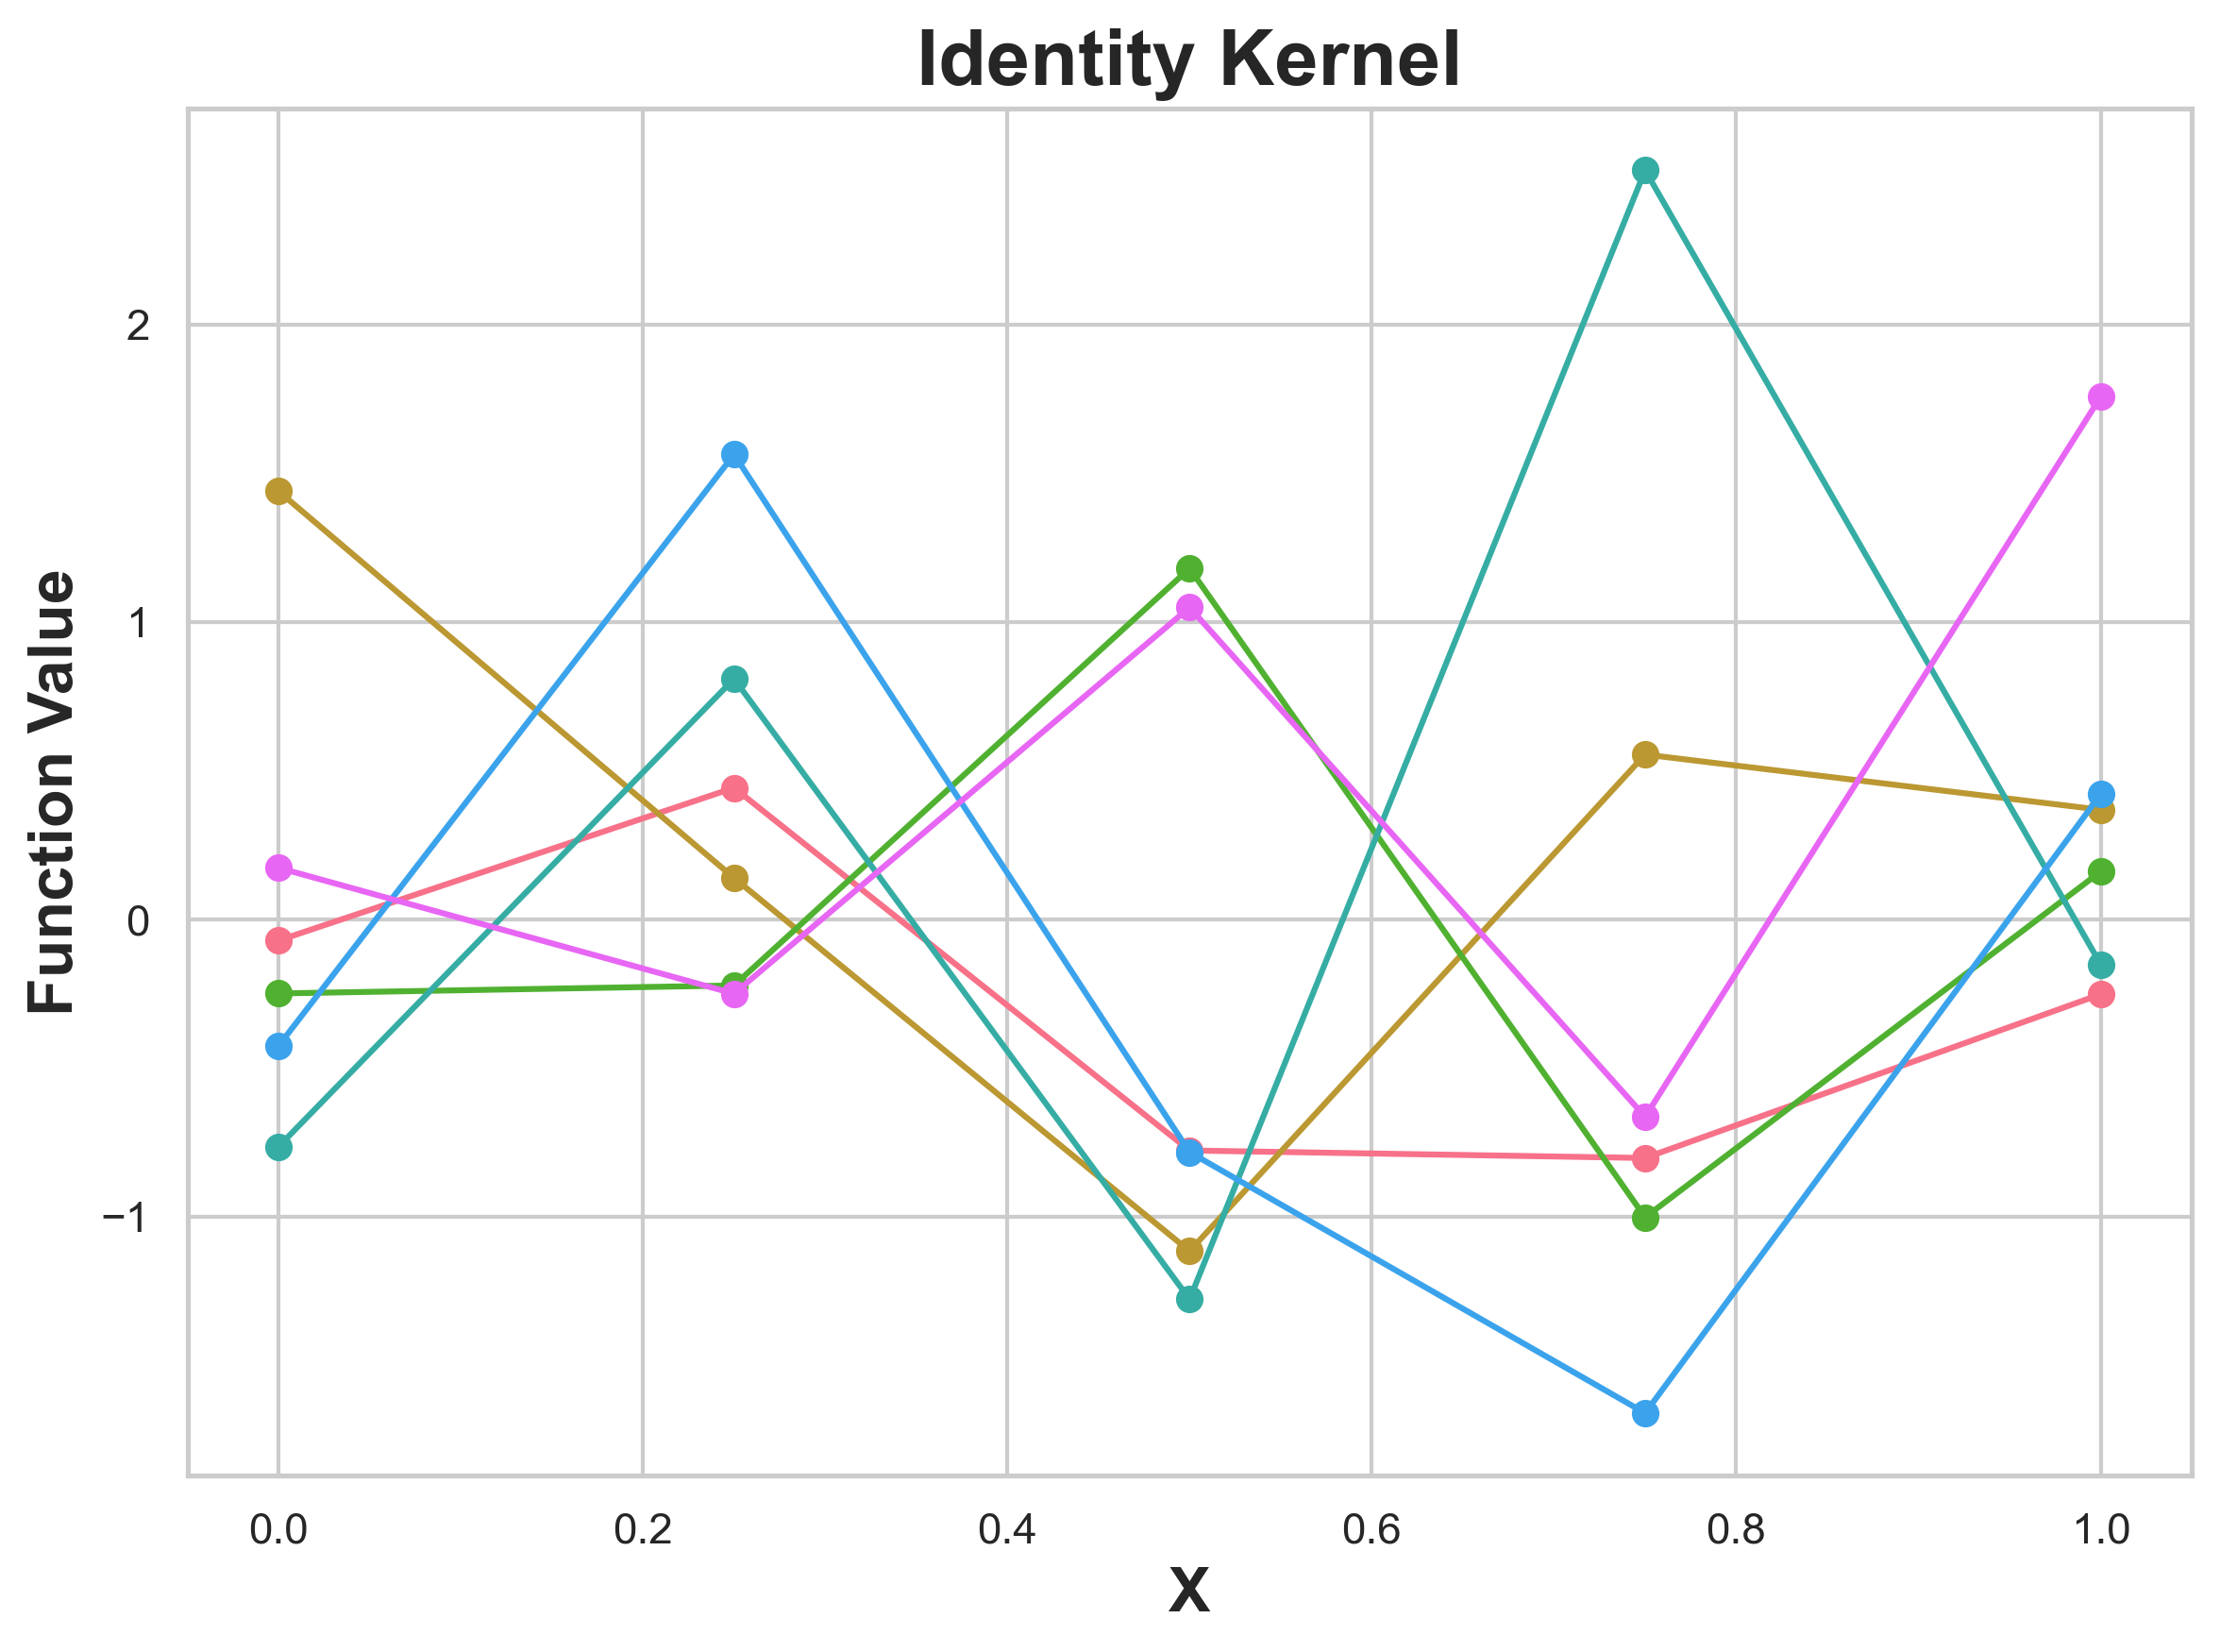
\includegraphics[width=\textwidth]{Images/Identity_Kernel.png}
%         \caption{First subplot}
%         \label{fig:sub1}
%     \end{subfigure}
%     \hfill
%     \begin{subfigure}[b]{0.32\textwidth}
%         \centering
%         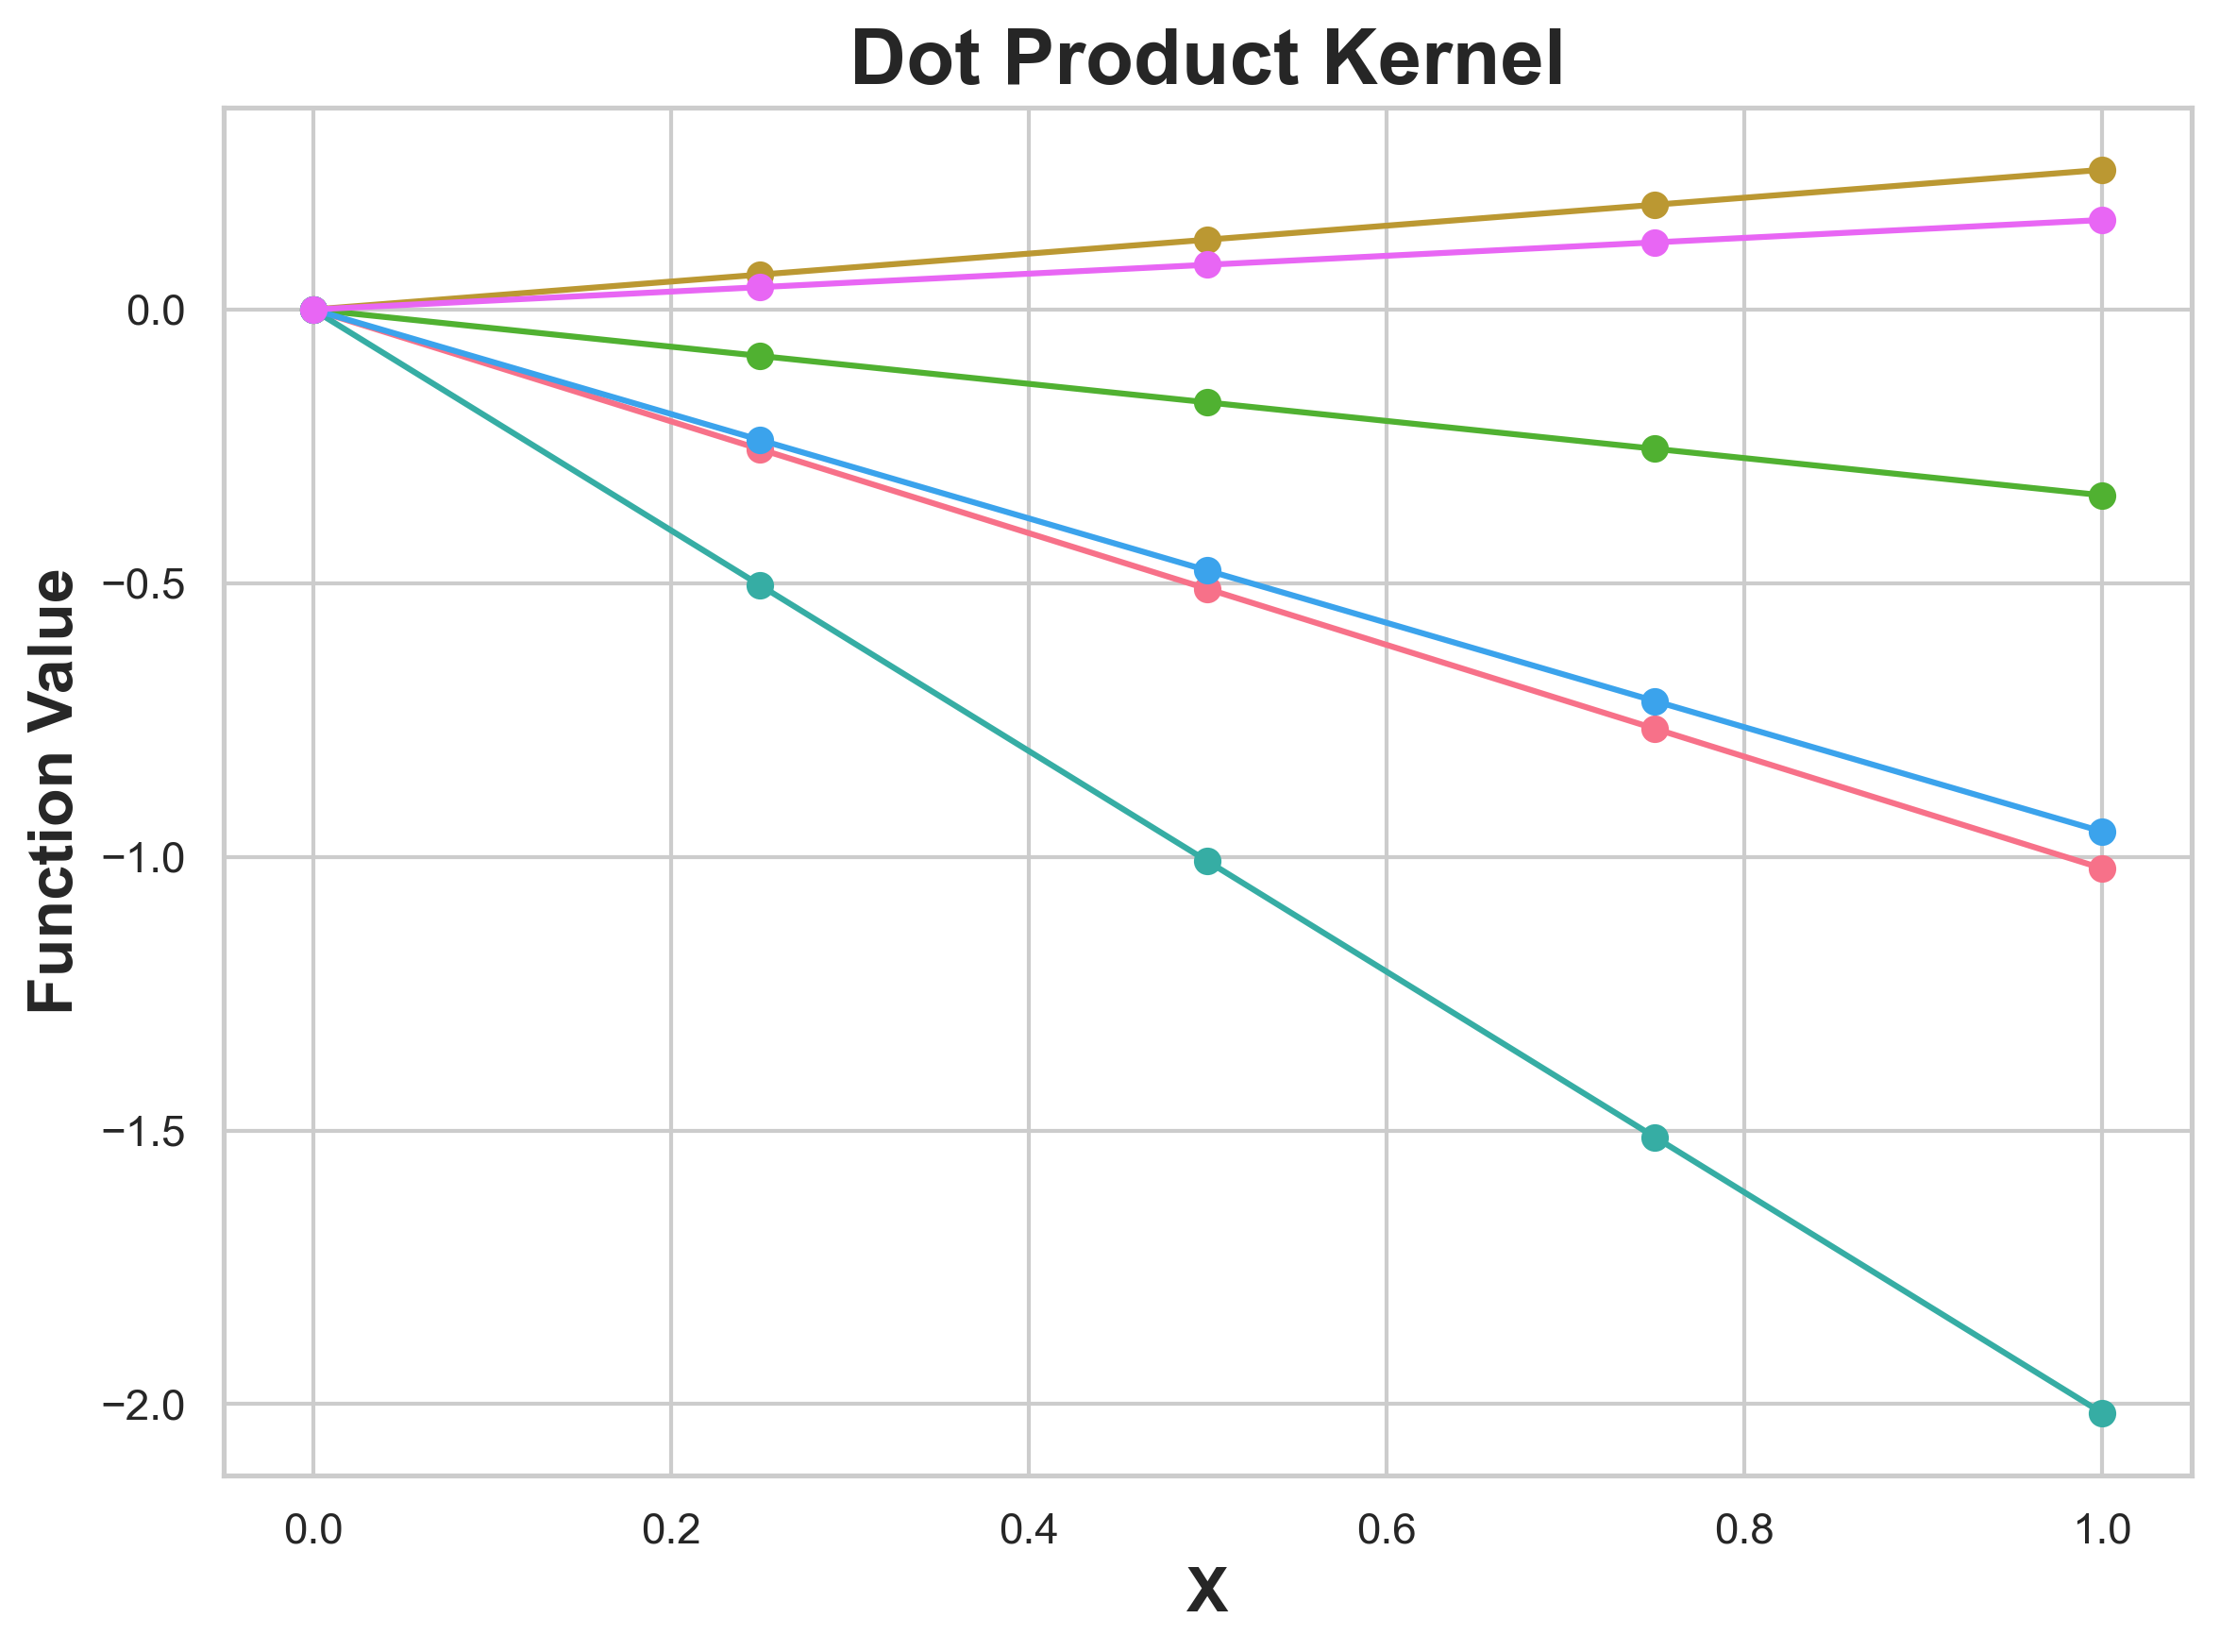
\includegraphics[width=\textwidth]{Images/Dot_Product_Kernel.png}
%         \caption{Second subplot}
%         \label{fig:sub2}
%     \end{subfigure}
%     \hfill
%     \begin{subfigure}[b]{0.32\textwidth}
%         \centering
%         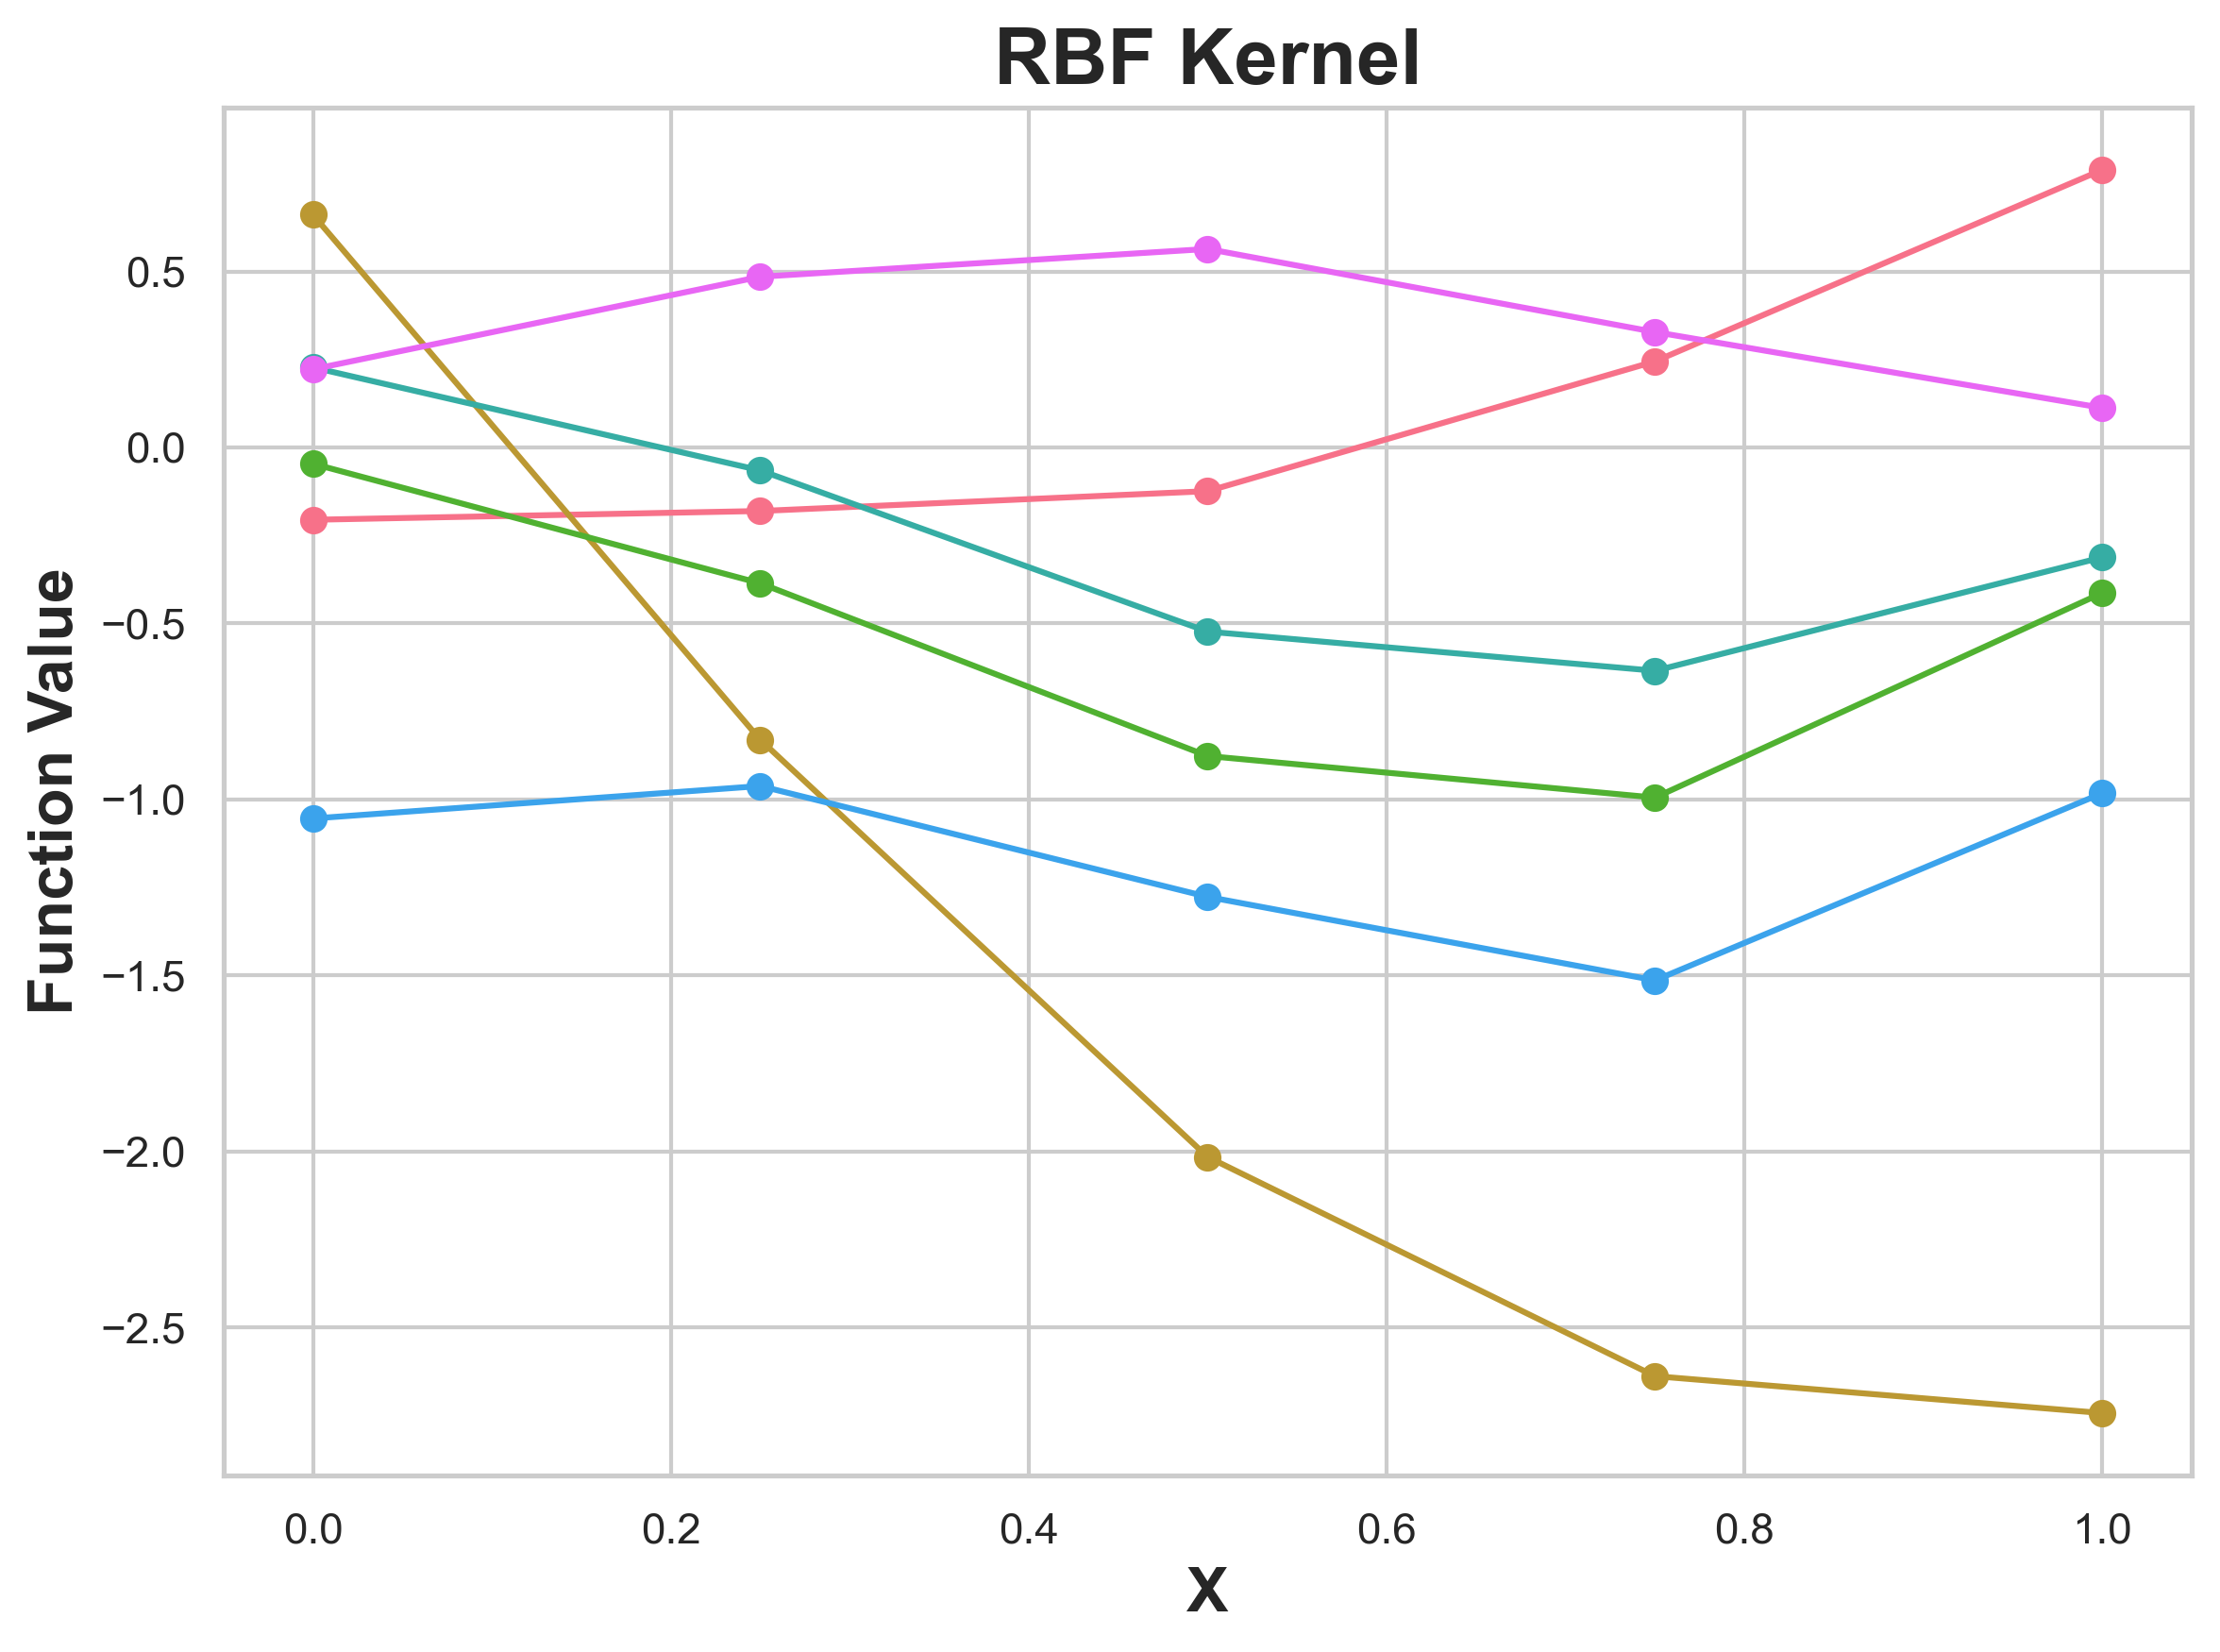
\includegraphics[width=\textwidth]{Images/RBF_Kernel.png}
%         \caption{Third subplot}
%         \label{fig:sub3}
%     \end{subfigure}
%     \caption{Samples from a normal multivariate distribution with zero mean and covariance defined by the Kernel}
%     \label{fig:subplots}
% \end{figure}

\subsection{Adding Data: Building the Posterior}

By conditioning our prior distribution on our training data (true data points), we build our posterior distribution from which we can make predictions. 

\noindent
The function values at test points are conditioned on the function values at training points:
\[
P(f_* | f, X, X_*).
\]
\noindent
Functionally, since the covariance structure already incorporates $X$ and $X_*$ through the kernel function, this reduces to computing:
\[
P(f(X_*) | f(X)).
\]
\noindent
Since we are dealing with continuous distributions, we have that the conditional probability is represented by the probability density function
$
p(f_* | f).
$
Using Bayes' Theorem applied to continuous probabilities, we have:
\[
p(f_* | f) = \frac{p(f_*, f)}{p(f)}.
\]
we have:
$$p(f_*,f) = \frac{1}{2\pi\sqrt{\mathbf{|C|}}}\exp \left(-\frac{1}{2} 
\begin{bmatrix} f \\ f_*  \end{bmatrix}^T\mathbf{C^{-1}}\begin{bmatrix} f  \\ f_* \end{bmatrix}\right)$$
and 
\[
p(f) = \frac{1}{\sqrt{2\pi} |K|^{1/2}}
\exp \left(-\frac{1}{2} f^T K^{-1} f \right).
\]

\noindent
\textbf{Legend:}
\begin{itemize}
    \item $K = K(X, X)$, $K_{**} = K(X_*,X_*)$, $K_* = K(X,x_*) = K(X_*,X)^T$
    \item $C = \begin{bmatrix}
K & K_* \\
K_*^T & K_{**}
\end{bmatrix}$
    \item $|\mathbf{C}| = K K_{**} - K_* K_*^T$: Determinant of the covariance matrix.
    \item $\mathbf{C^{-1}} = \frac{1}{|\mathbf{C}|} 
    \begin{bmatrix}
    K_{**} & -K_* \\ -K_*^T & K
    \end{bmatrix}$
    \item $m(X) = m(X_*) = 0$
\end{itemize}

\noindent


\noindent
We get out (do out in appendix): 
\[
p(f_* | f) = \frac{1}{\sqrt{2\pi} |K_{**} - K_*^T K^{-1} K_*|^{1/2}}
\exp \left(-\frac{1}{2} f_*^T (K_{**} - K_*^T K^{-1} K_*)^{-1}f_* \right).
\]
Since this follows a multivariate Gaussian distribution, we write:

\[
p(f_* | f) \sim \mathcal{N}(m(f_*), \text{Var}(f_*)).
\]
where:
\[
m(f_*) = K_*^T K^{-1}f .
\]
\[
\text{Var}(f_*) = K_{**} - K_*^T K^{-1} K_*.
\]


\subsection{Graphical Representation of prior to posterior}
% \begin{figure}[ht]
%     \centering
%     \begin{tikzpicture}
%         % First image (shifted further left)
%         \node[anchor=south west] (img1) at (-4.5,0) 
%             {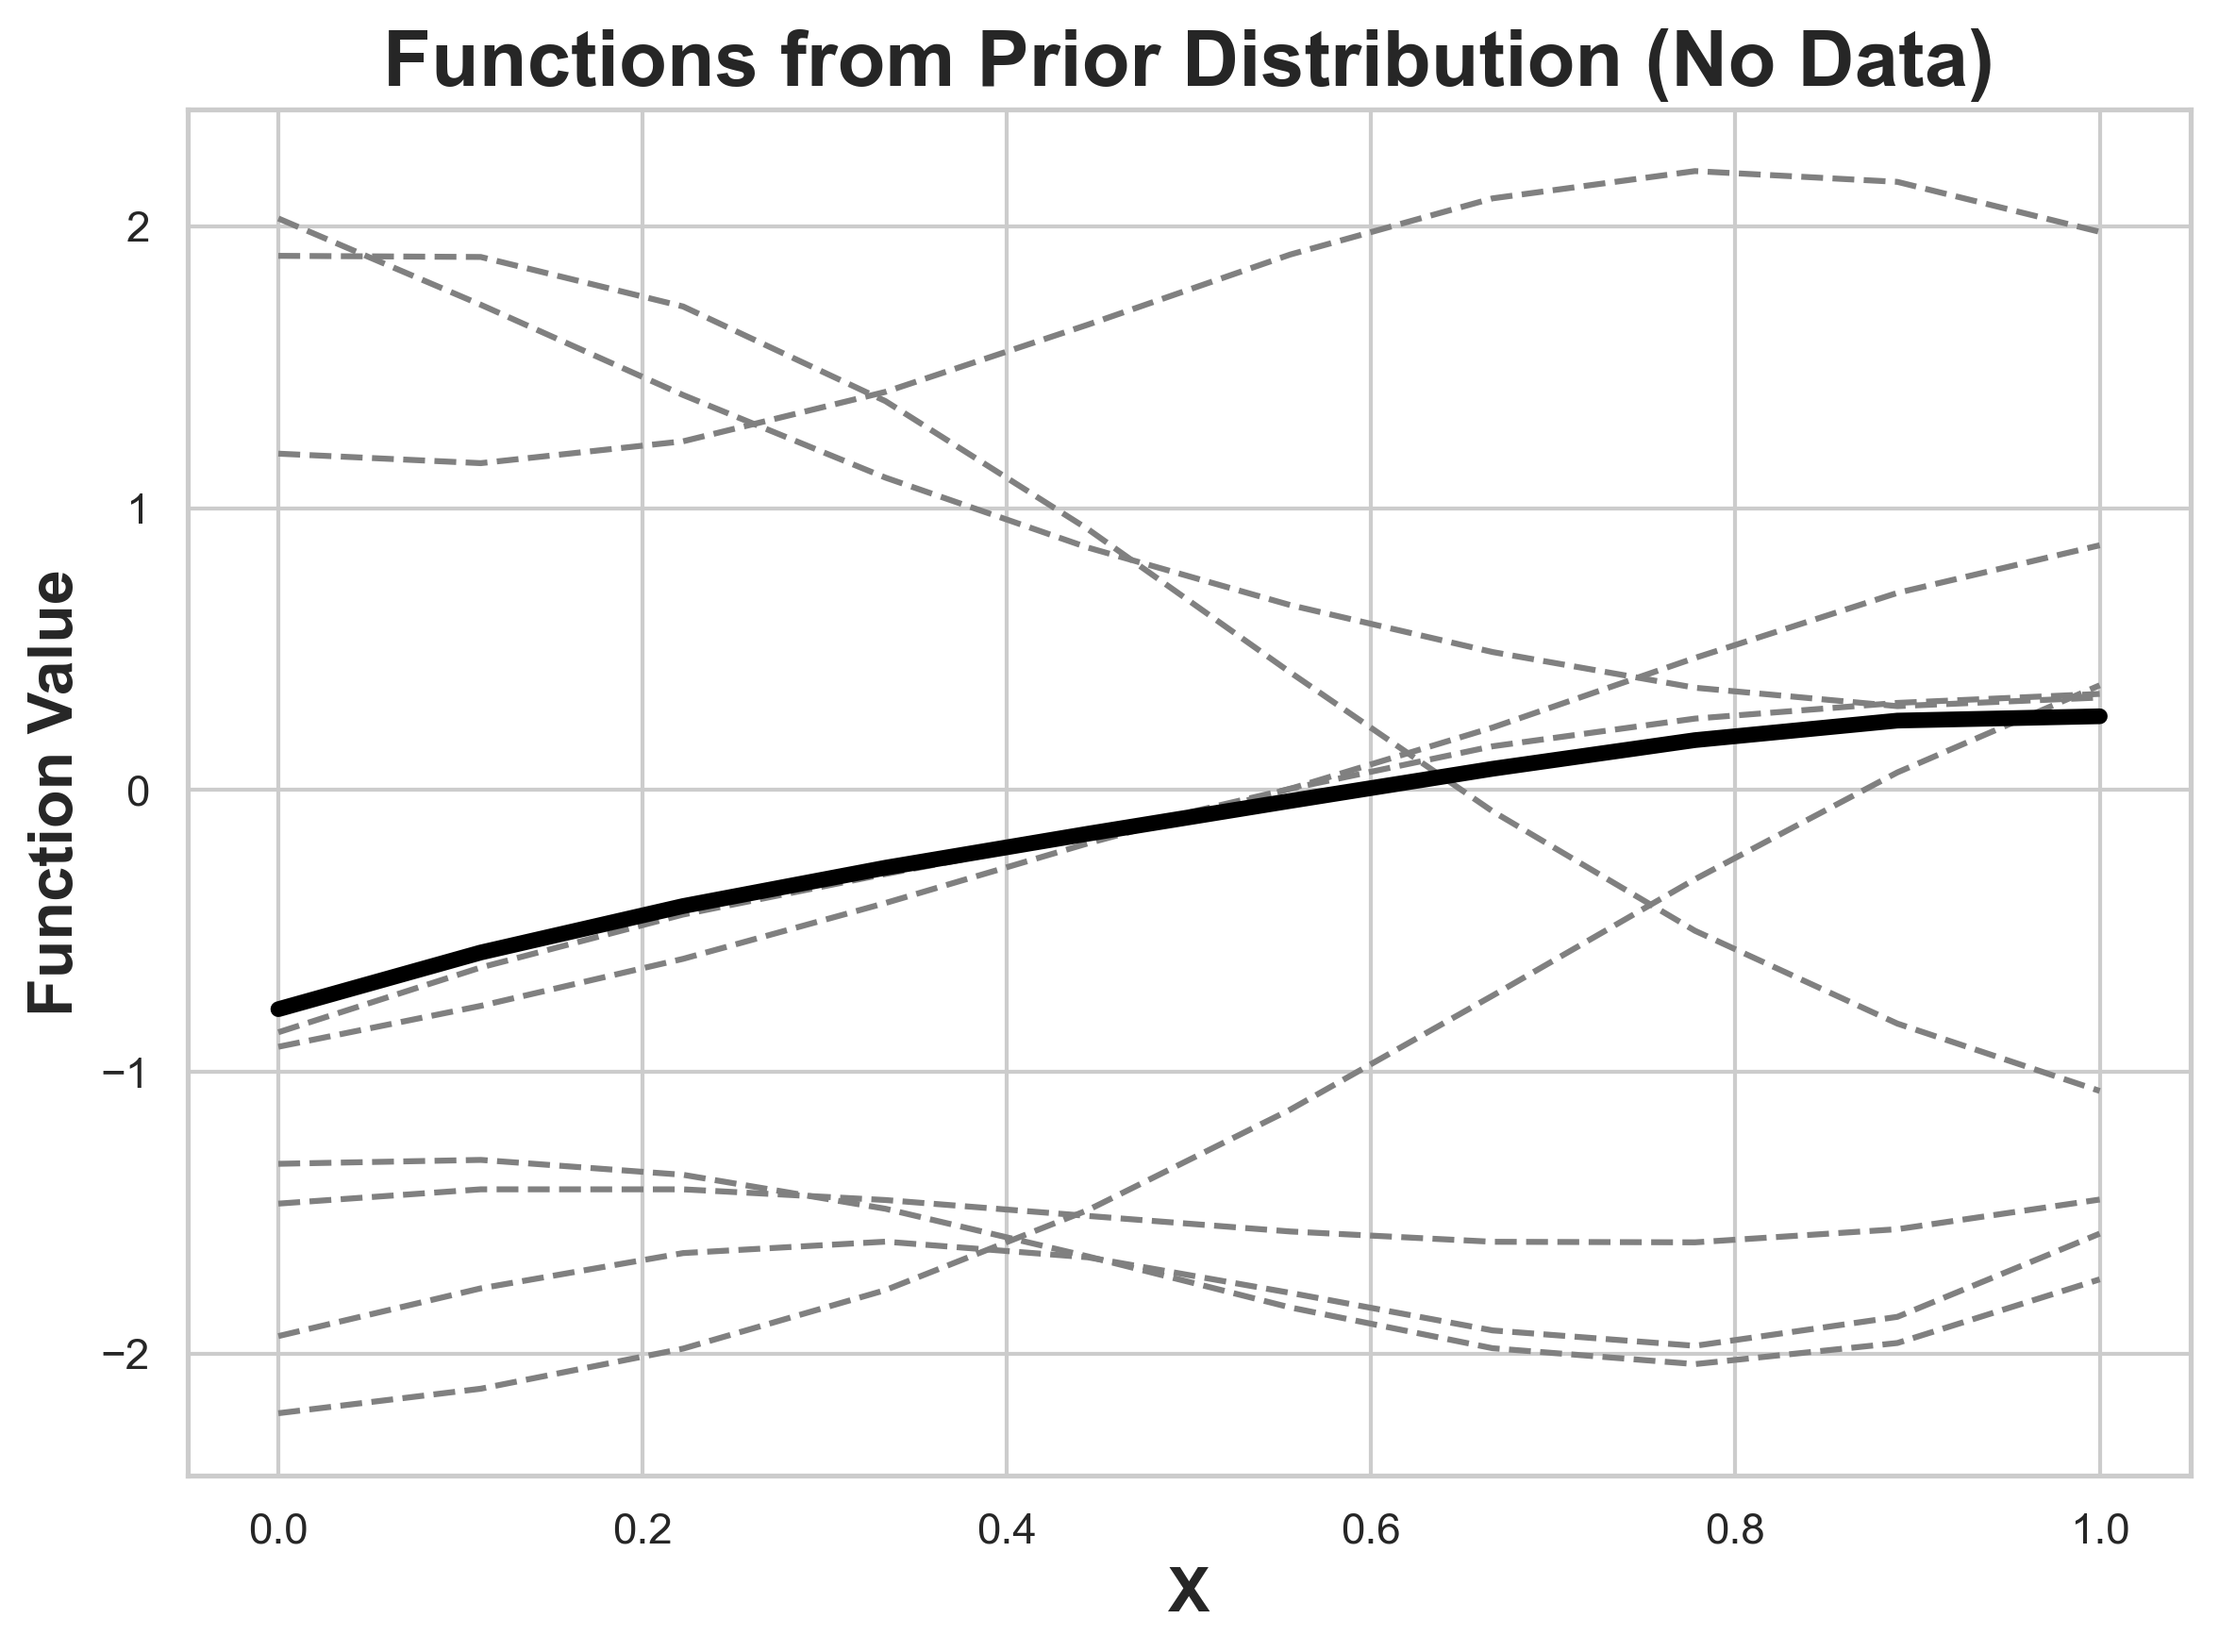
\includegraphics[width=0.35\textwidth]{Images/prior_distribution.png}};
        
%         % Arrow 1 (shifted left)
%         \node at (0.5,1.5) {\LARGE $\rightarrow$};
        
%         % Second image (shifted further left)
%         \node[anchor=south west] (img2) at (1,0) 
%             {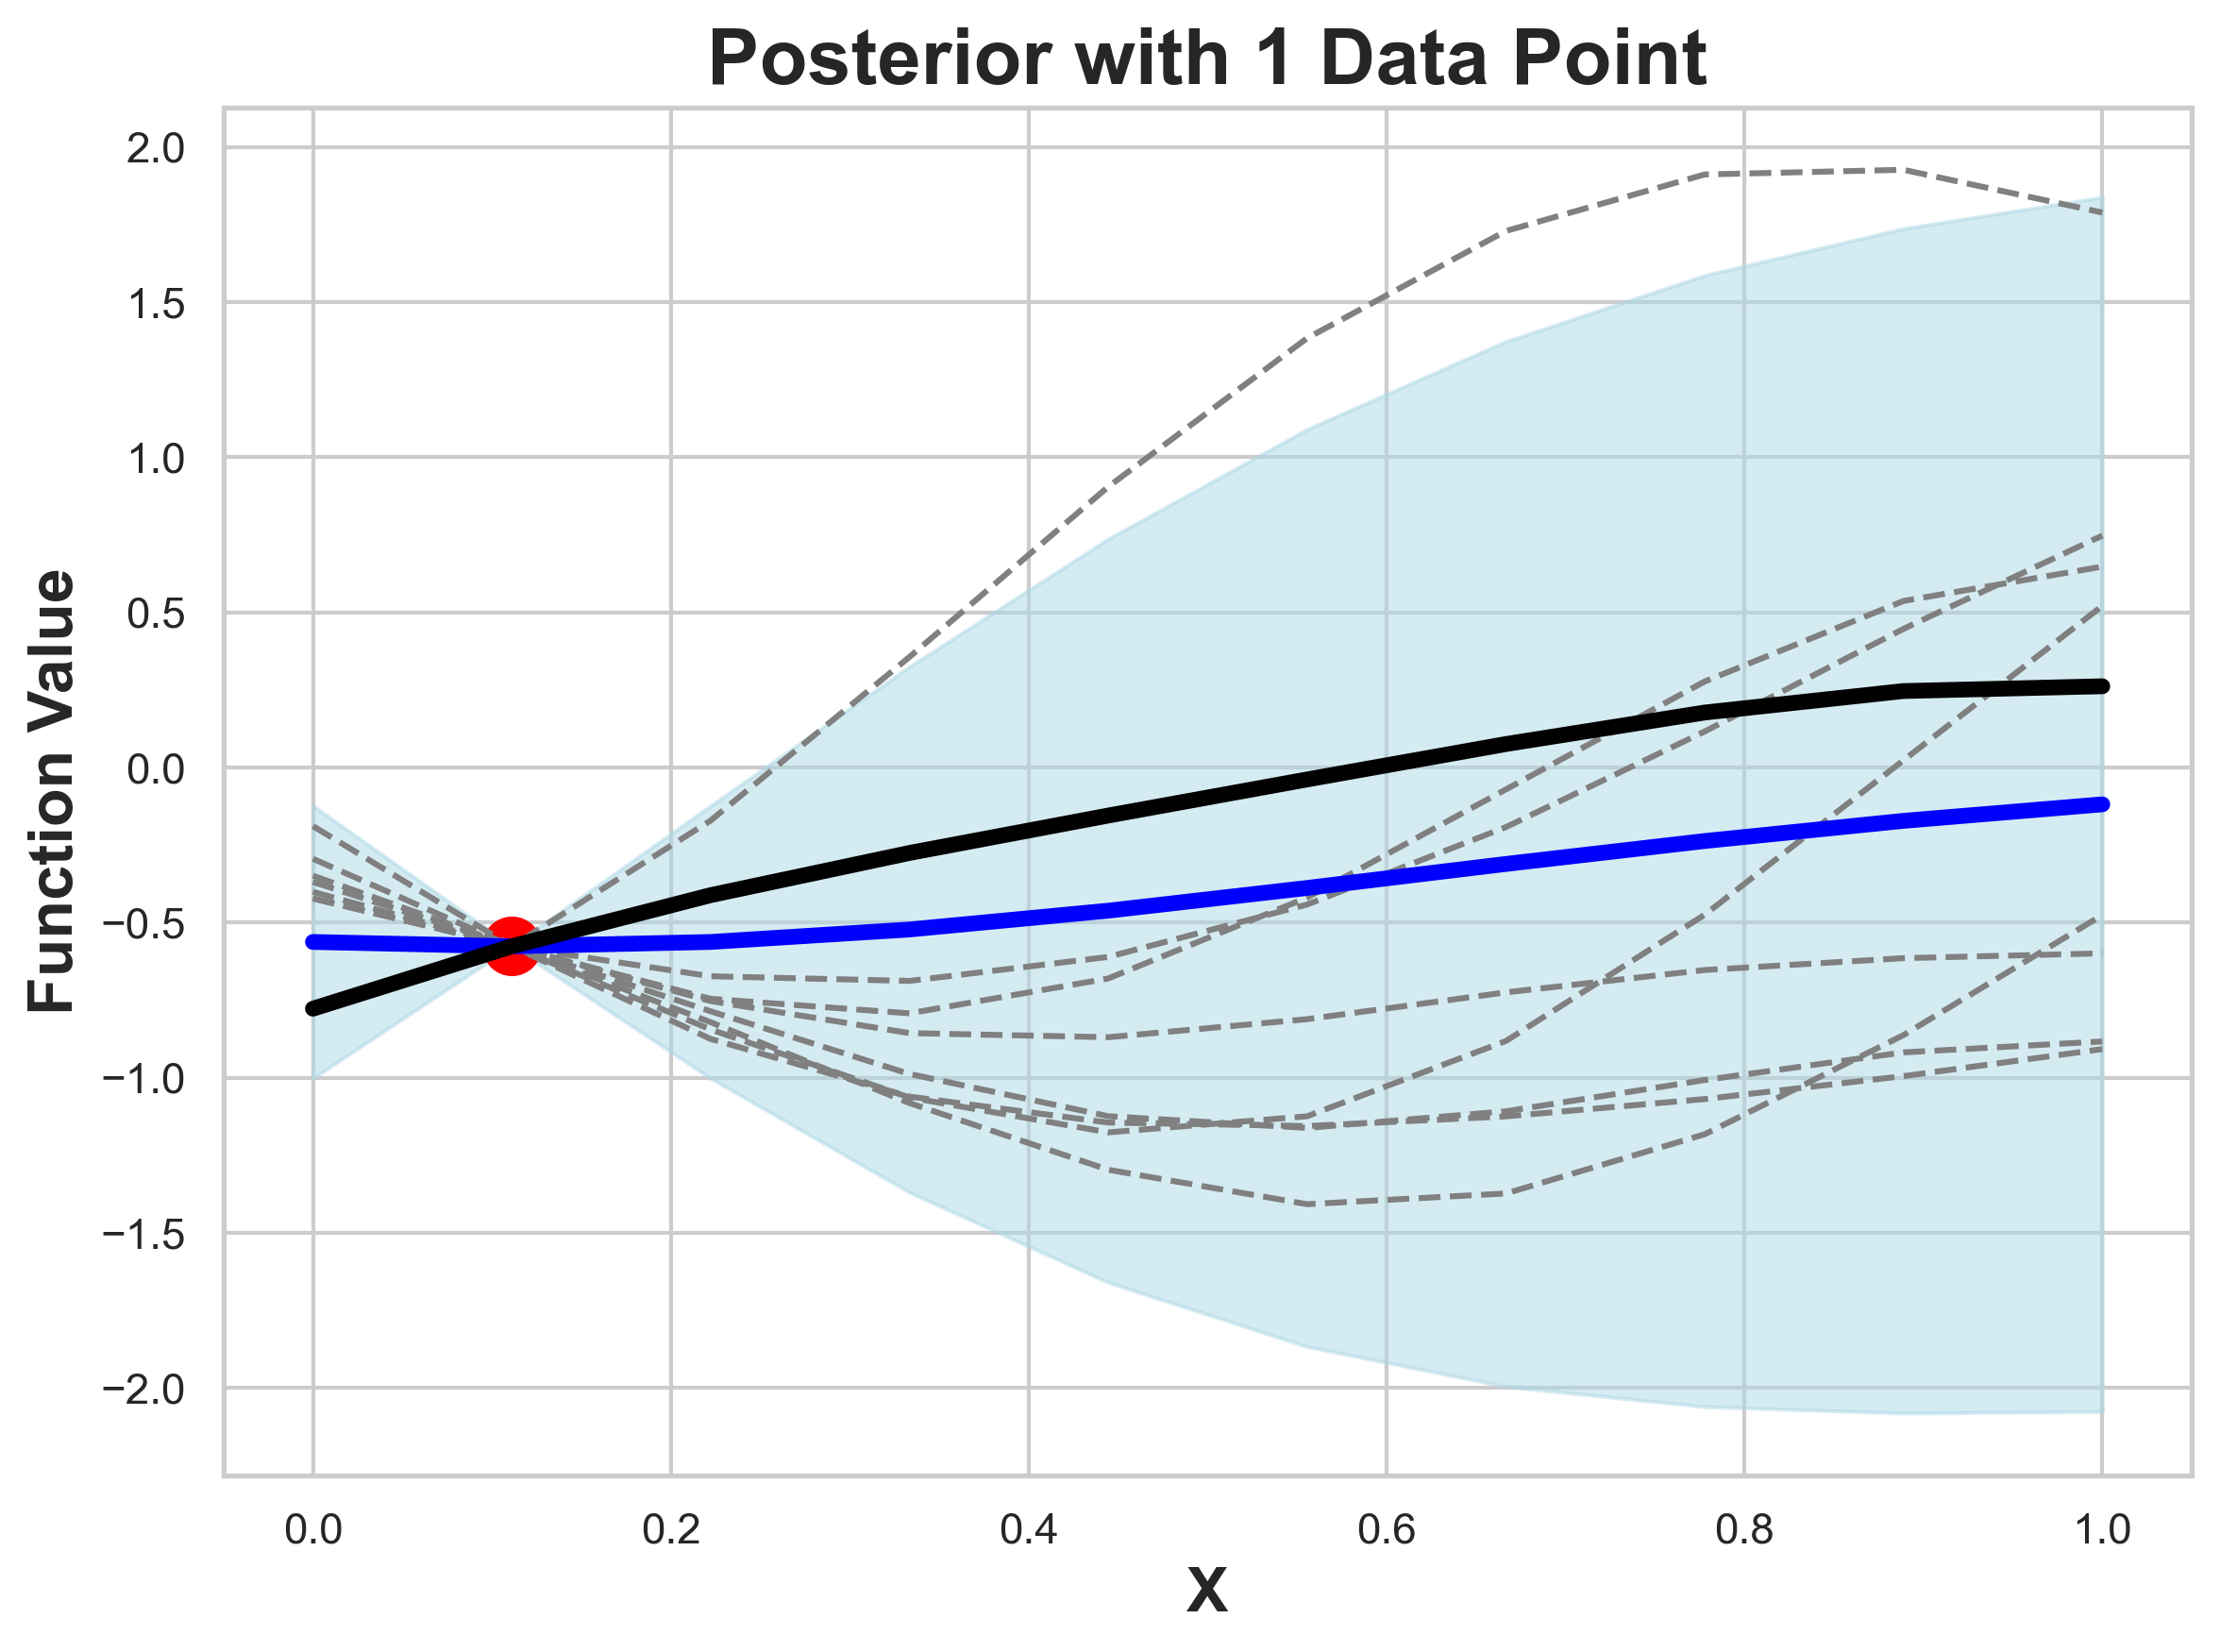
\includegraphics[width=0.35\textwidth]{Images/posterior_1_point.png}};
        
%         % Arrow 2 (shifted left)
%         \node at (6,1.5) {\LARGE $\rightarrow$};
        
%         % Third image (shifted further left)
%         \node[anchor=south west] (img3) at (6.5,0) 
%             {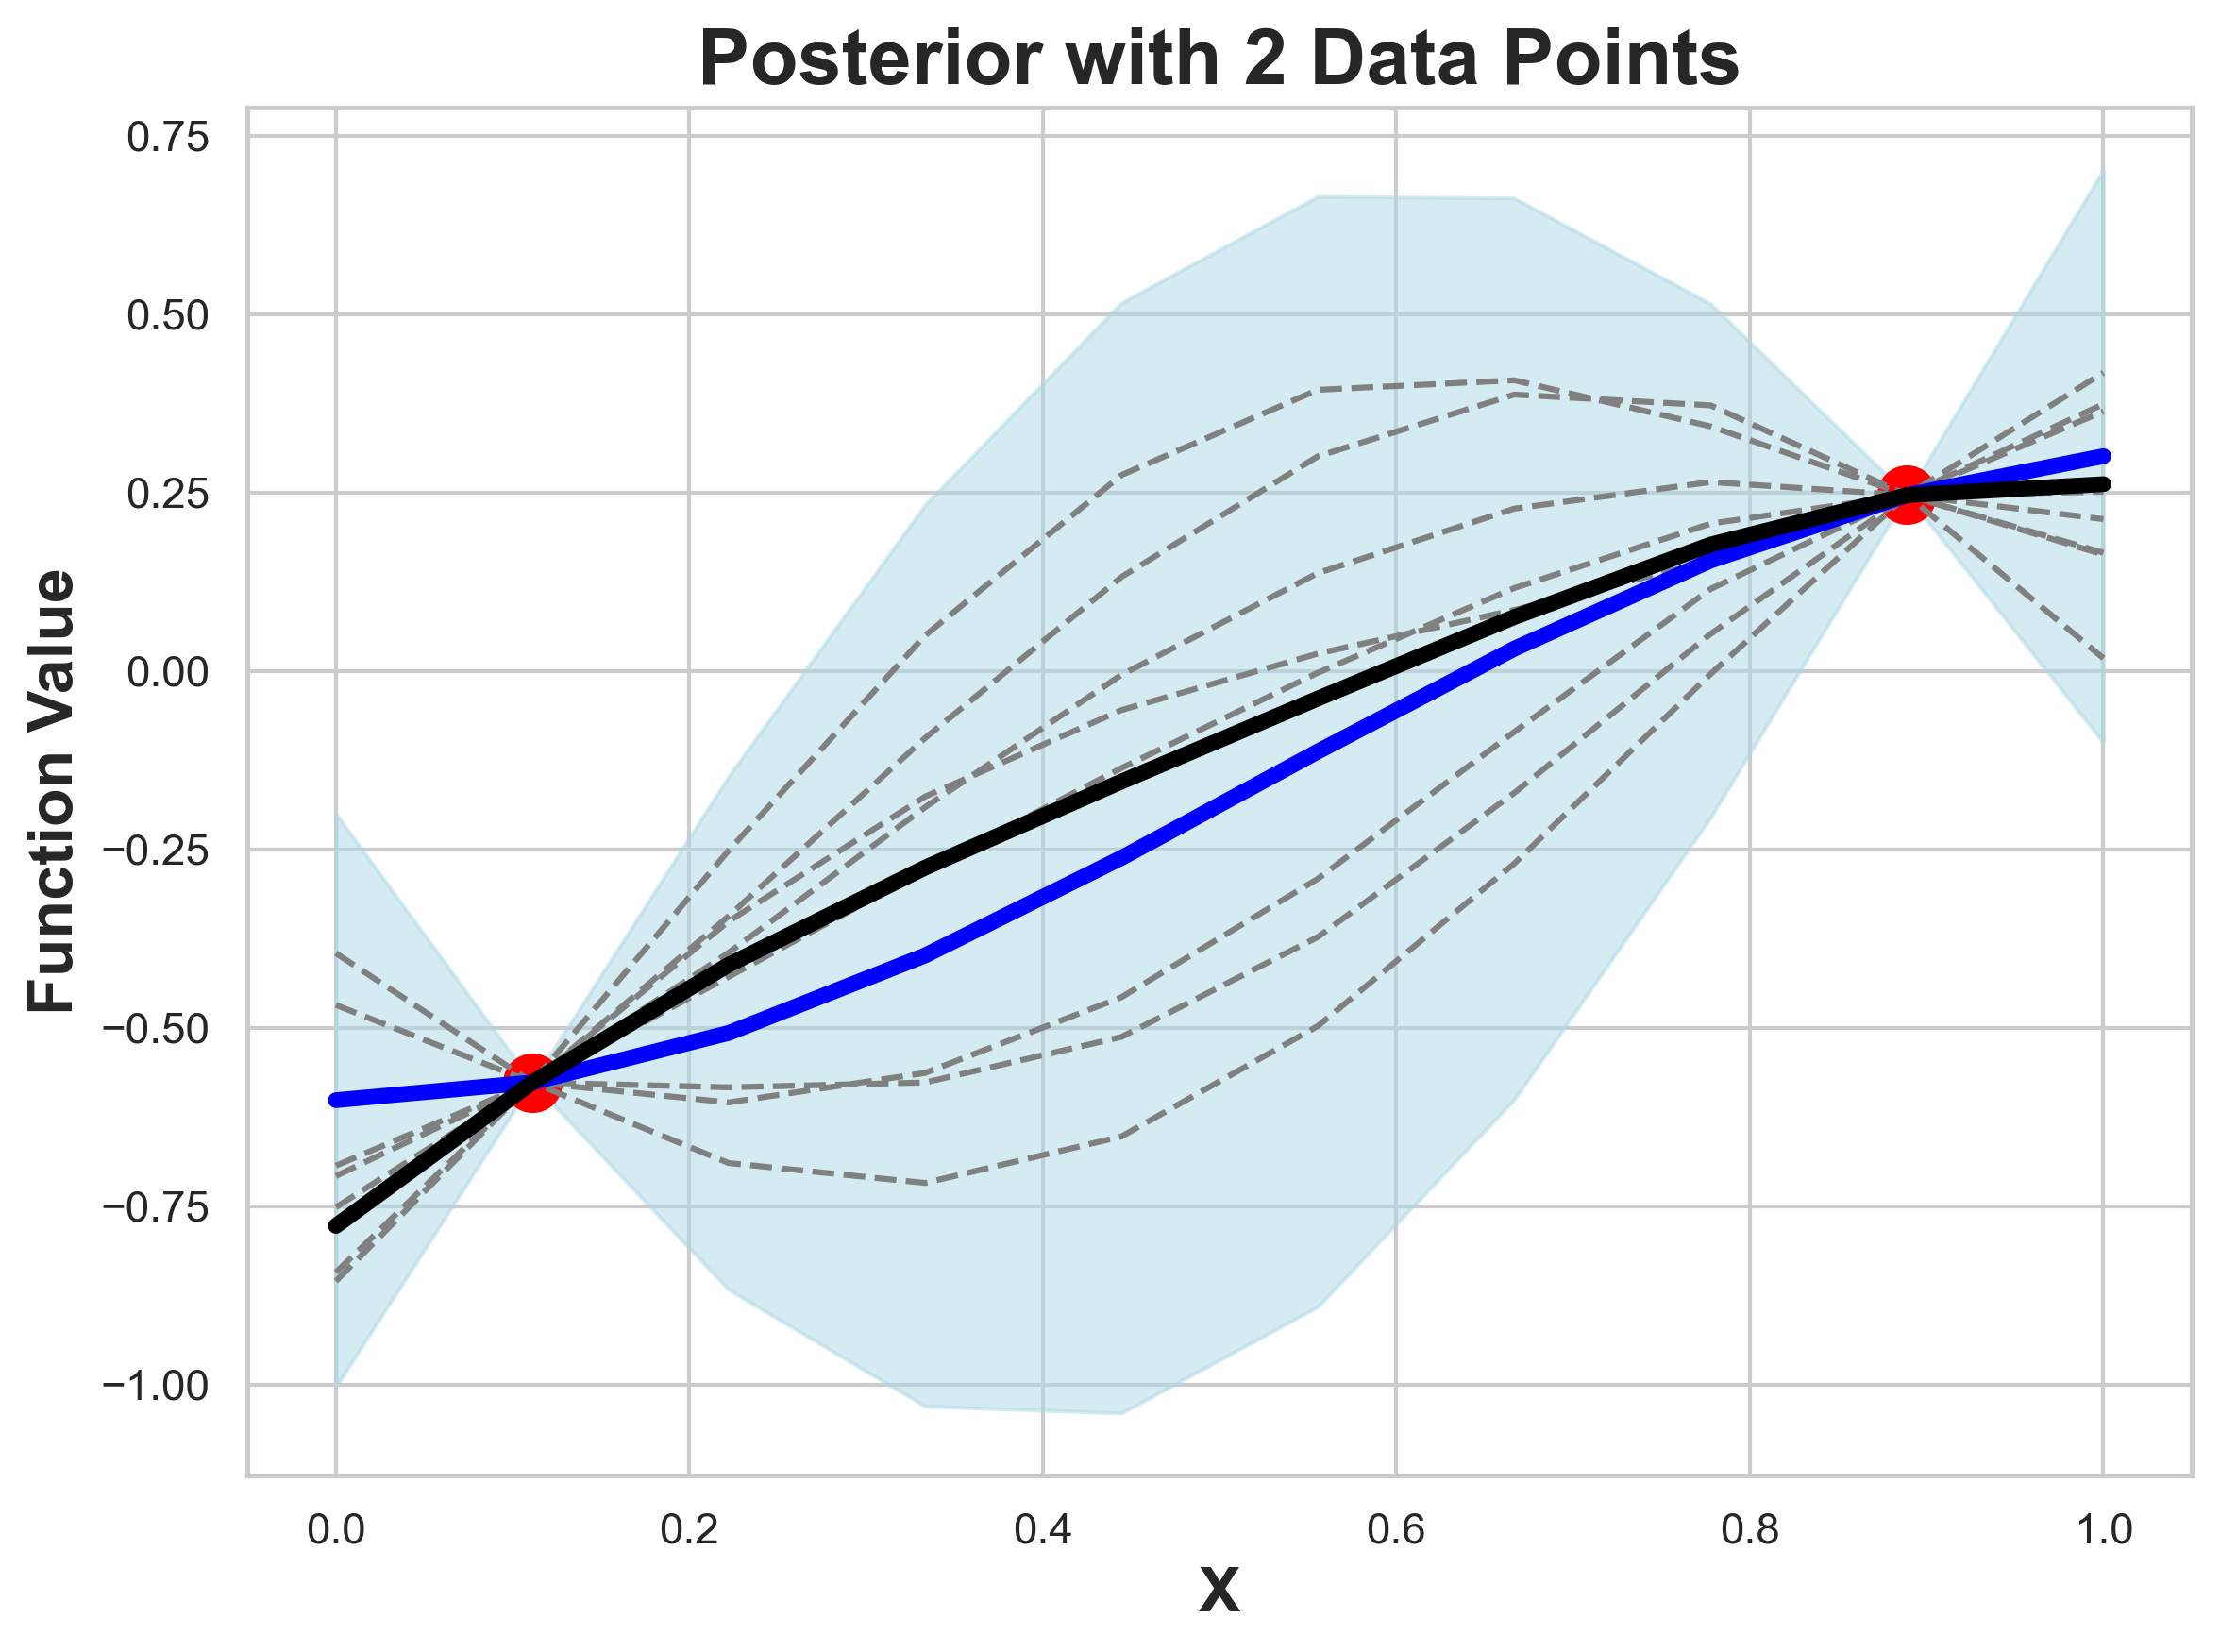
\includegraphics[width=0.35\textwidth]{Images/posterior_2_points.png}};
%     \end{tikzpicture}
%     \caption{Transition from prior to posterior as more data points are added.}
%     \label{fig:prior_to_posterior}
% \end{figure}



\subsection{Hyper-parameter Optimisation}

We have seen how we condition our prior on data with kernel funtion. But we can optimise our hyper-parameters to find the best fitting posterior distribution.


% \begin{figure}[h]
%     \centering
%     \begin{subfigure}[b]{0.45\textwidth}
%         \centering
%         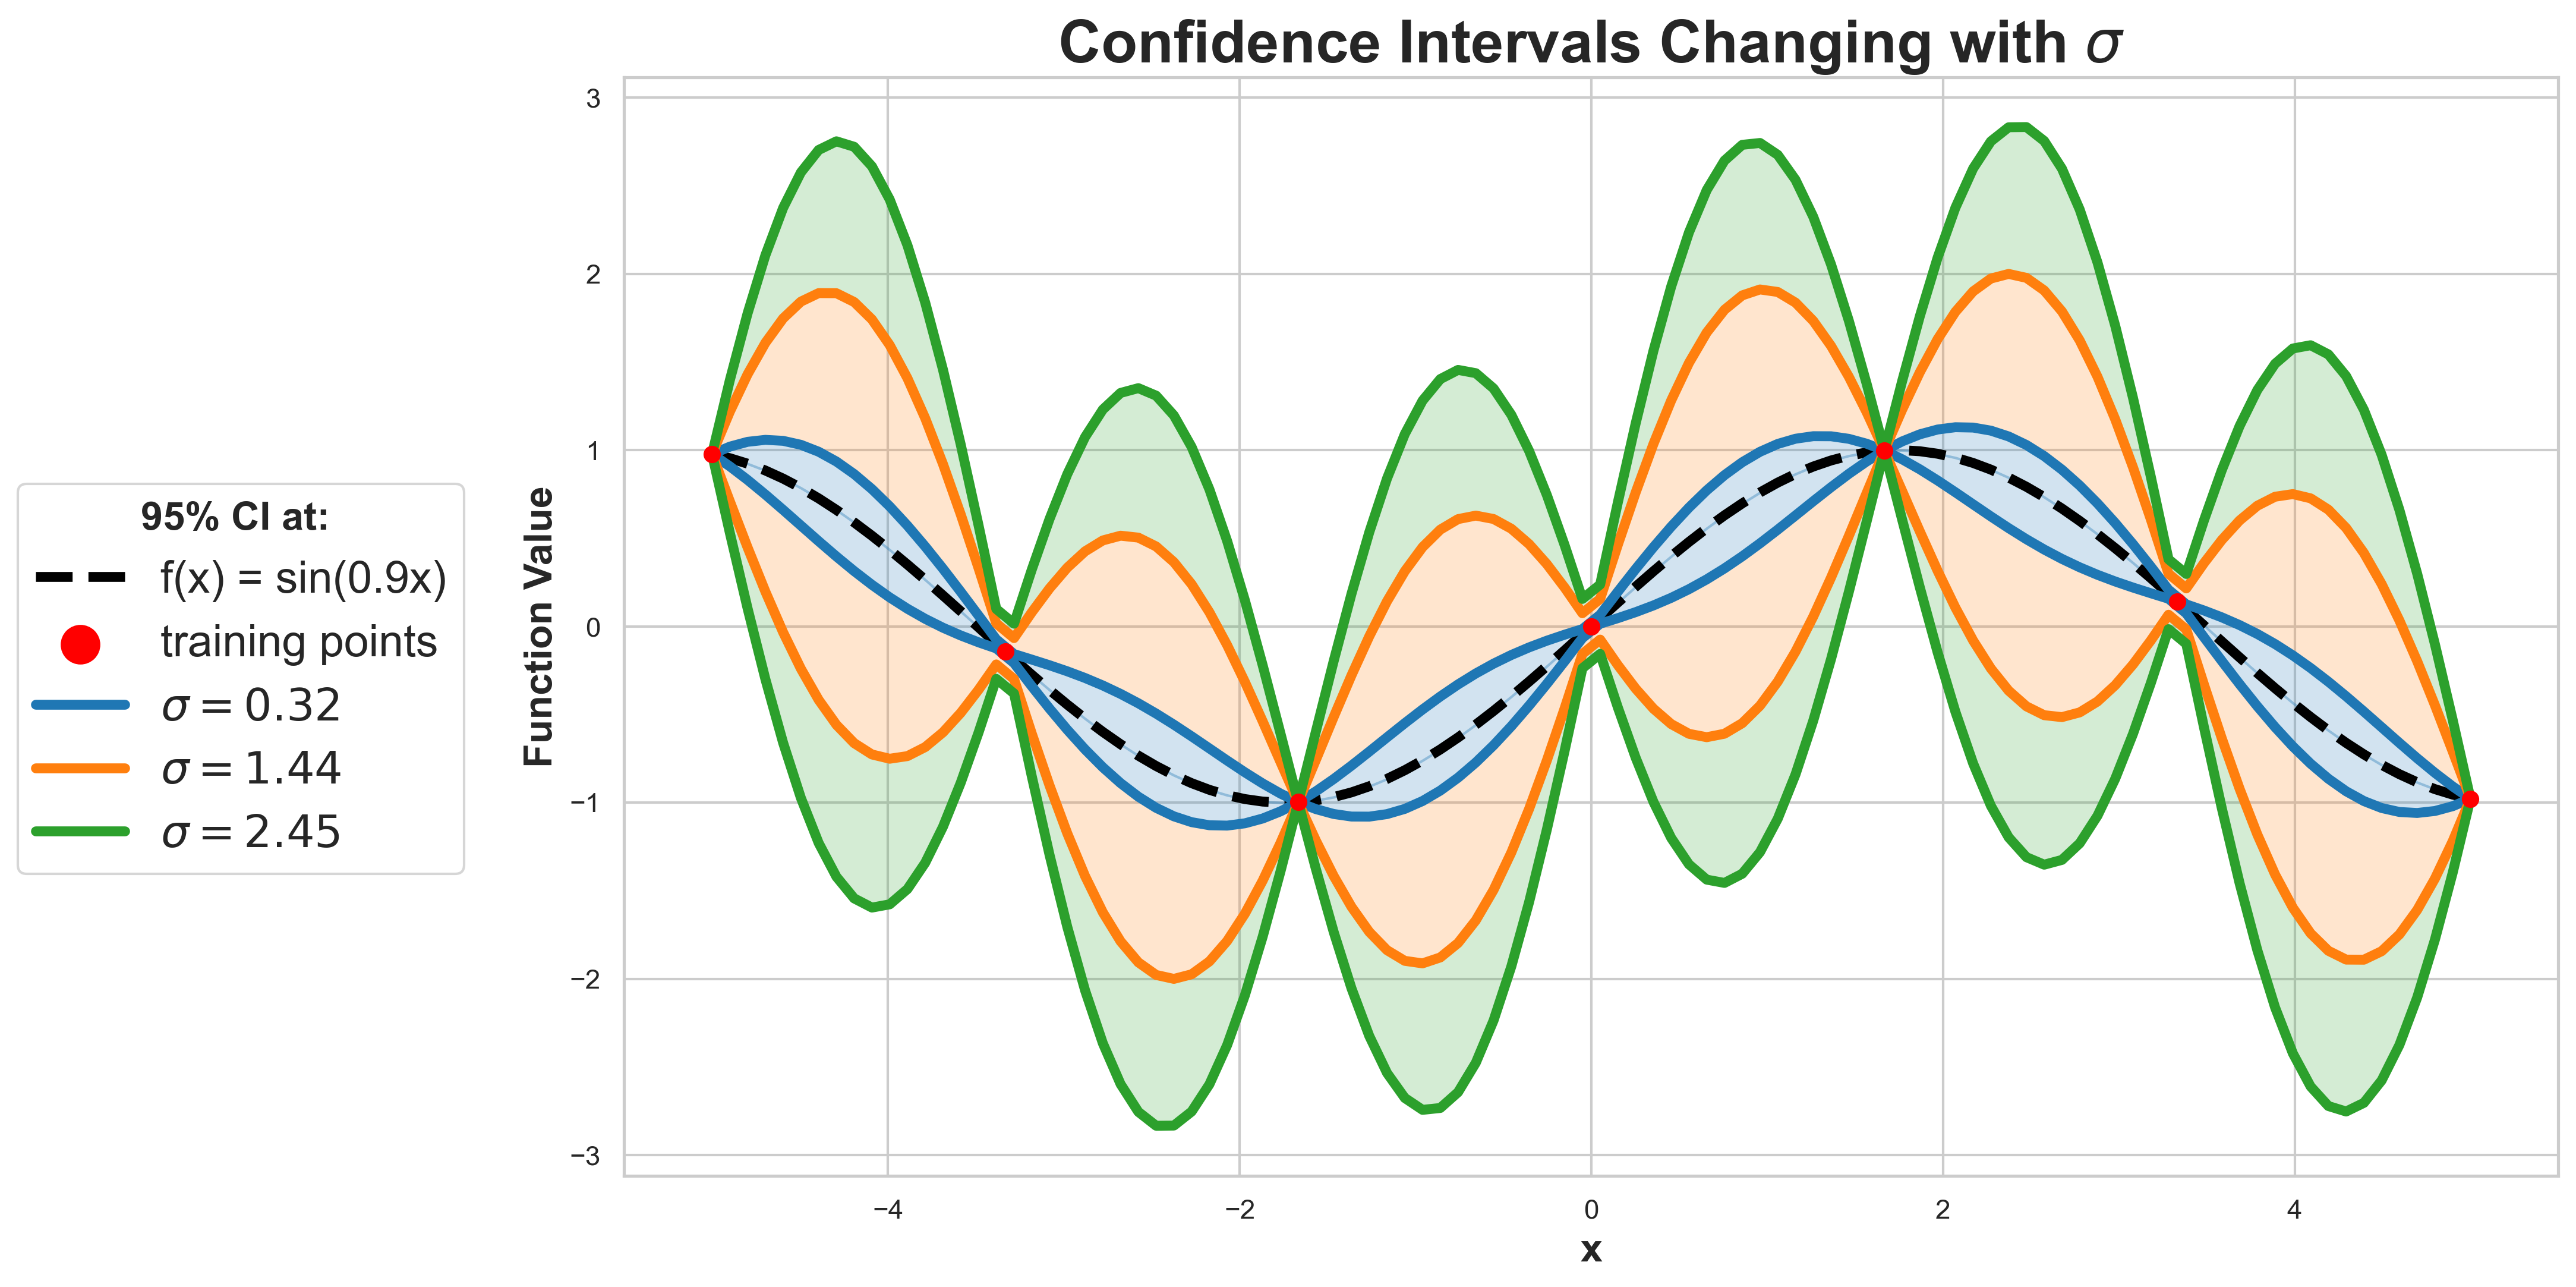
\includegraphics[width=\textwidth]{Images/Confidence_Intervals_Changing_with_Variance.png}
%         \caption{First subplot}
%         \label{fig:sub1}
%     \end{subfigure}
%     \hfill
%     \begin{subfigure}[b]{0.45\textwidth}
%         \centering
%         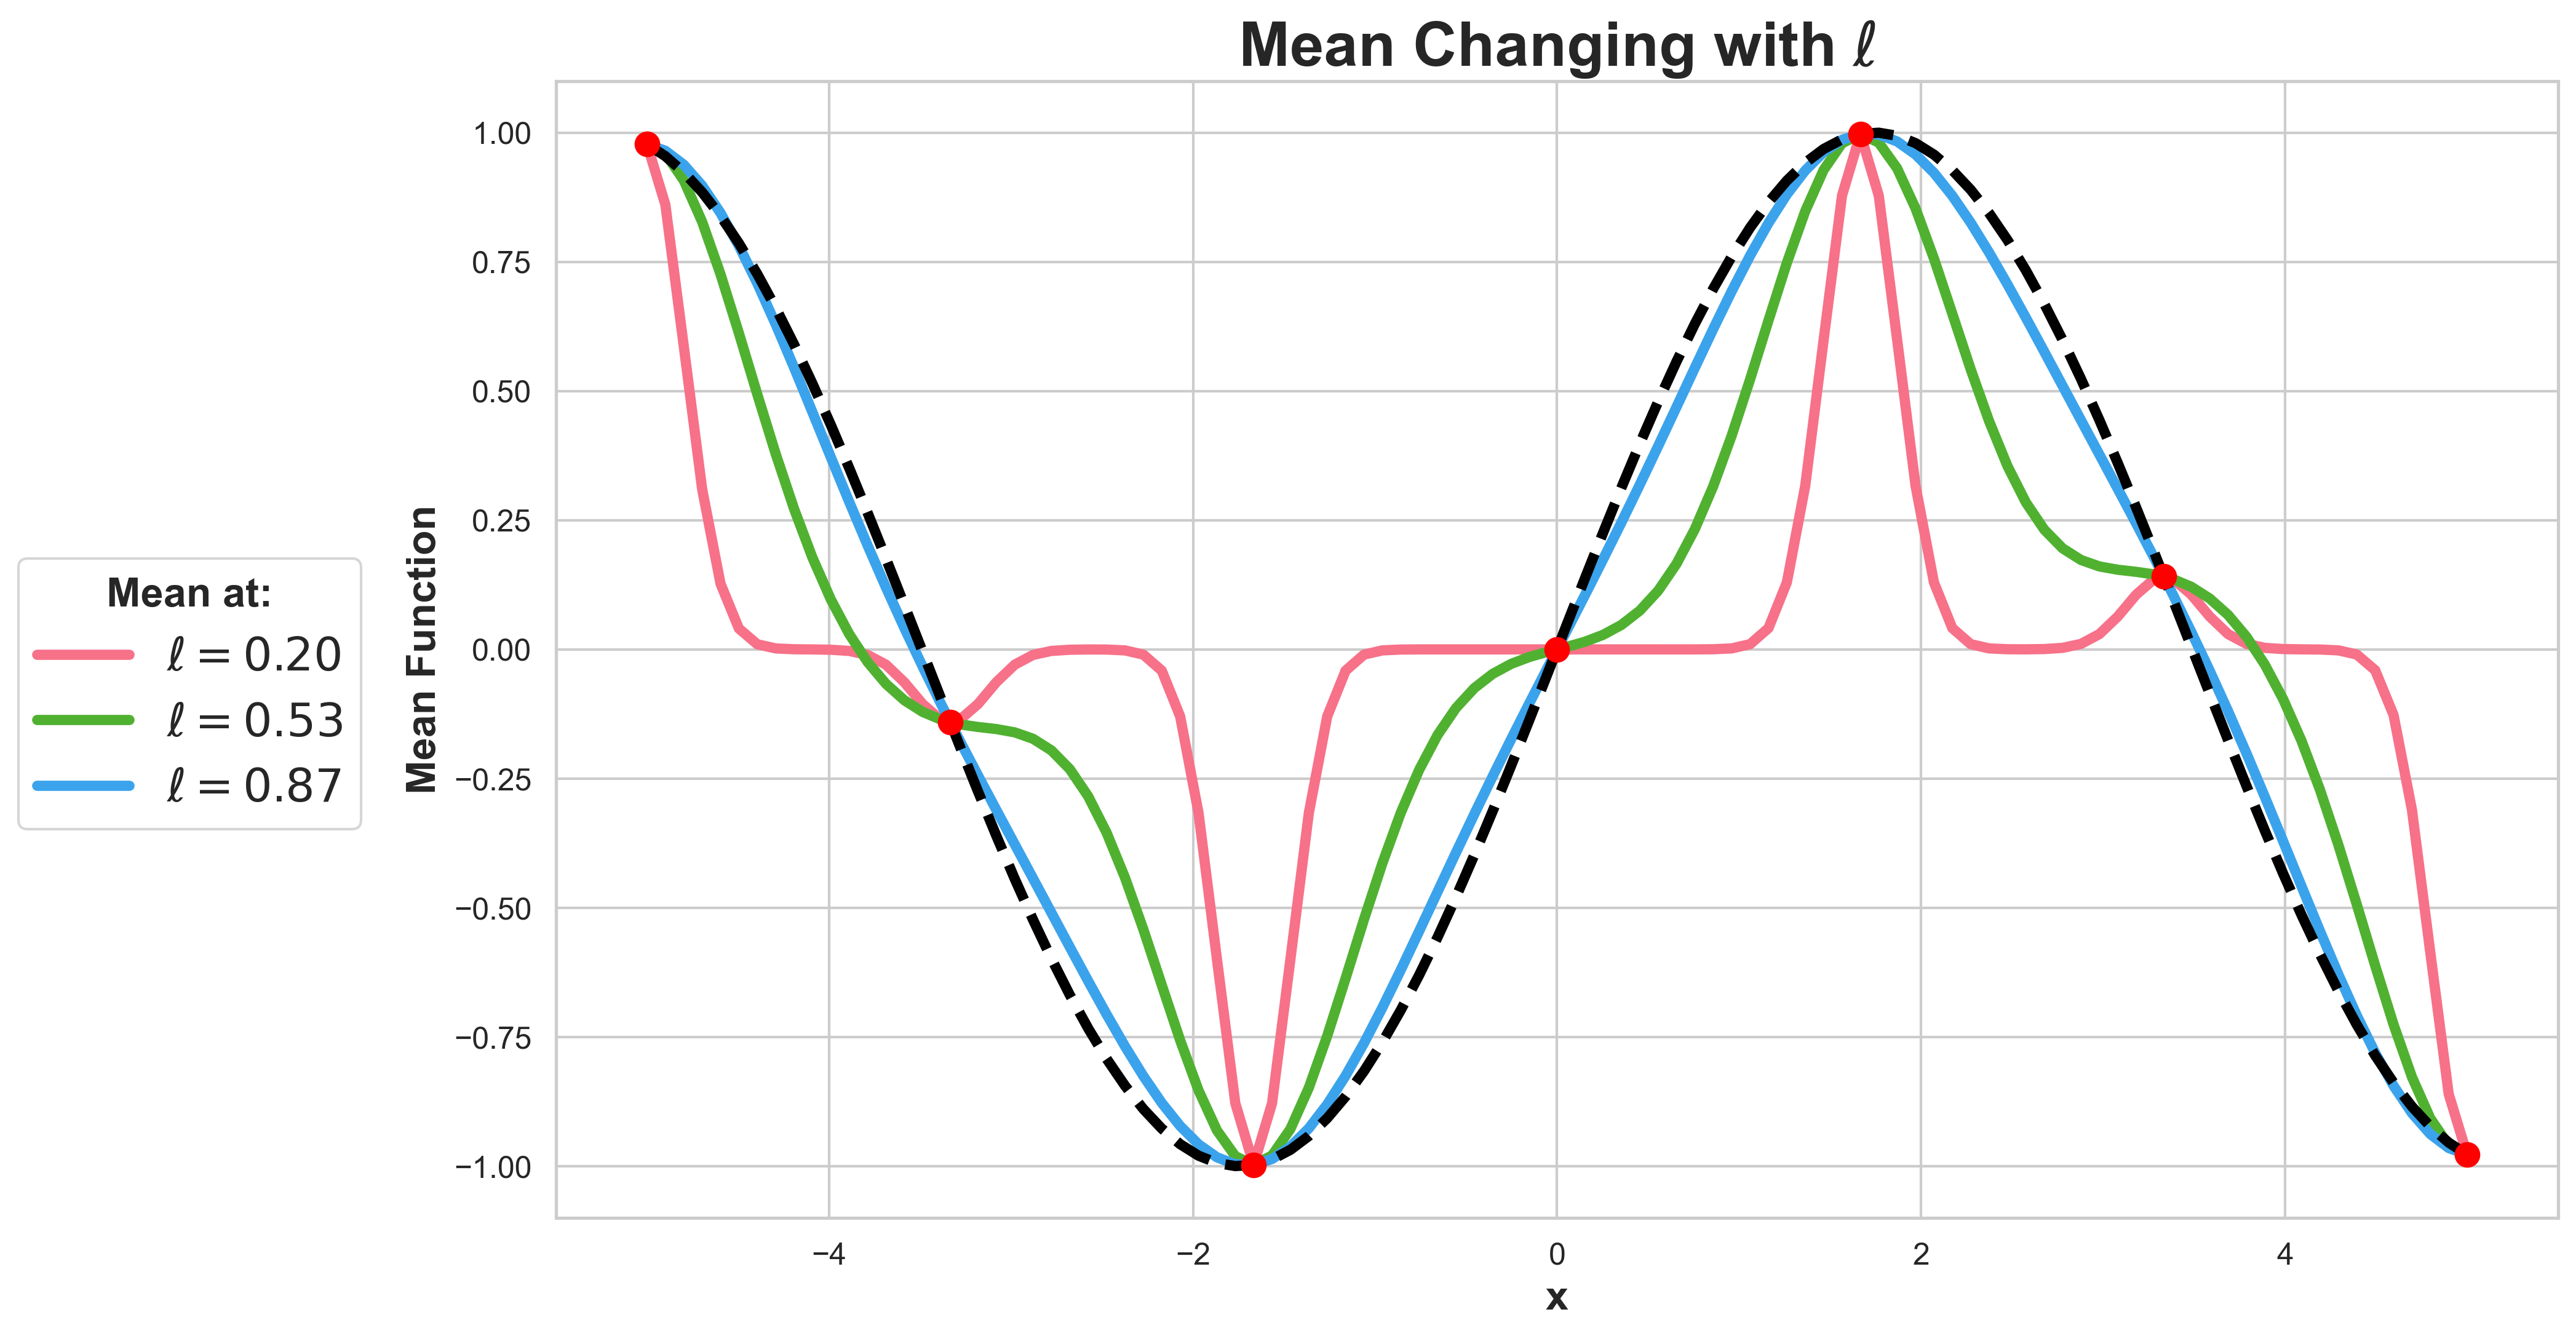
\includegraphics[width=\textwidth]{Images/Mean_Changing_with_Length.png}
%         \caption{Second subplot}
%         \label{fig:sub2}
%     \end{subfigure}
%     \caption{How the kernel effects the posterior distribution. Make sure to change confidence interval to credible interval}
%     \label{fig:subplots}
% \end{figure}

\noindent
Done by log-likelihood and L2 norm cross validation


\section{Next steps for results}

\begin{itemize}
     \item Find a scientific approach and well justifiable reason on what kernel was picked and for what reasons.
     \item Use Different Cross Validation and optimising techniques and again find a justifiable reason on which one performs best and for what reasons.
     \item Include the variance in the Kernel hyper-parameters into my posterior. Accounts for more general results, less effected by noise
    \item Compare under computational cost and accuracy the model done in different dimensional spaces. 4d,7d,8d.
    \item Run these different models on other mismatch data from other functional fit and interpolant models to find which model generalizes best.
    \item justify 4 dimensional hyper-parameters
\end{itemize}


\section{Kernels}

\section{Different Models}
\begin{itemize}
    \item White Kernel without Error Knowledge
    \item White Kenrel With Error Knowledge
    \item Using $\alpha = err^2$
    \item Using Monte Carlo Sampling, Sampling from the Error
    \item Using MCMCing to build a posterior on hyper-parameter distribution
    \item Picking values from this posterior distribution to use
\end{itemize}

\section{Choosing the Best Performing Model take performance and Efficiency into account}

\subsection{Kernel Selection}

% \begin{figure}[H]  % 'H' forces the figure to appear exactly here
%     \centering
%     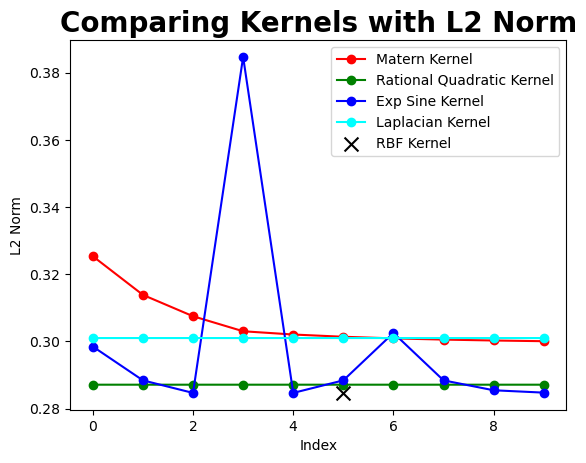
\includegraphics[width=0.6\textwidth]{GoodPlots/KernelL2norms.png}  % Change to your image filename
%     \caption{Plotting the L2norm of the posterior predictions for different Kernels}
%     \label{fig:my_graph}
% \end{figure}

% \begin{figure}[H]  % 'H' forces the figure to appear exactly here
%     \centering
%     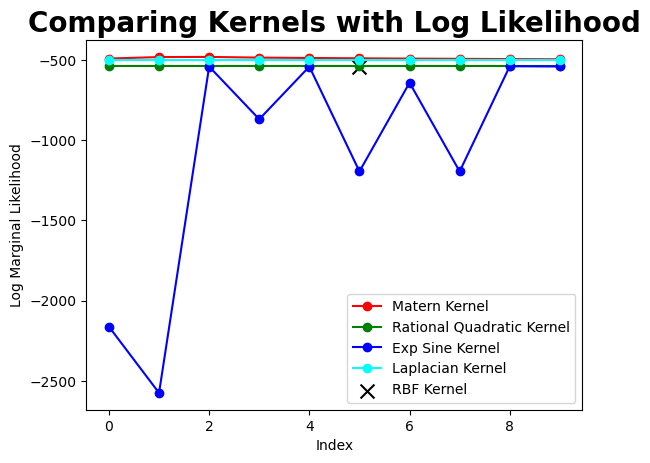
\includegraphics[width=0.6\textwidth]{GoodPlots/LogLikeKernels.png}  % Change to your image filename
%     \caption{Plotting the Log likelihood for different Kernels}
%     \label{fig:my_graph}
% \end{figure}


% \subsection{Different Posterior Building Techniques}

% \begin{figure}[H]  % 'H' forces the figure to appear exactly here
%     \centering
%     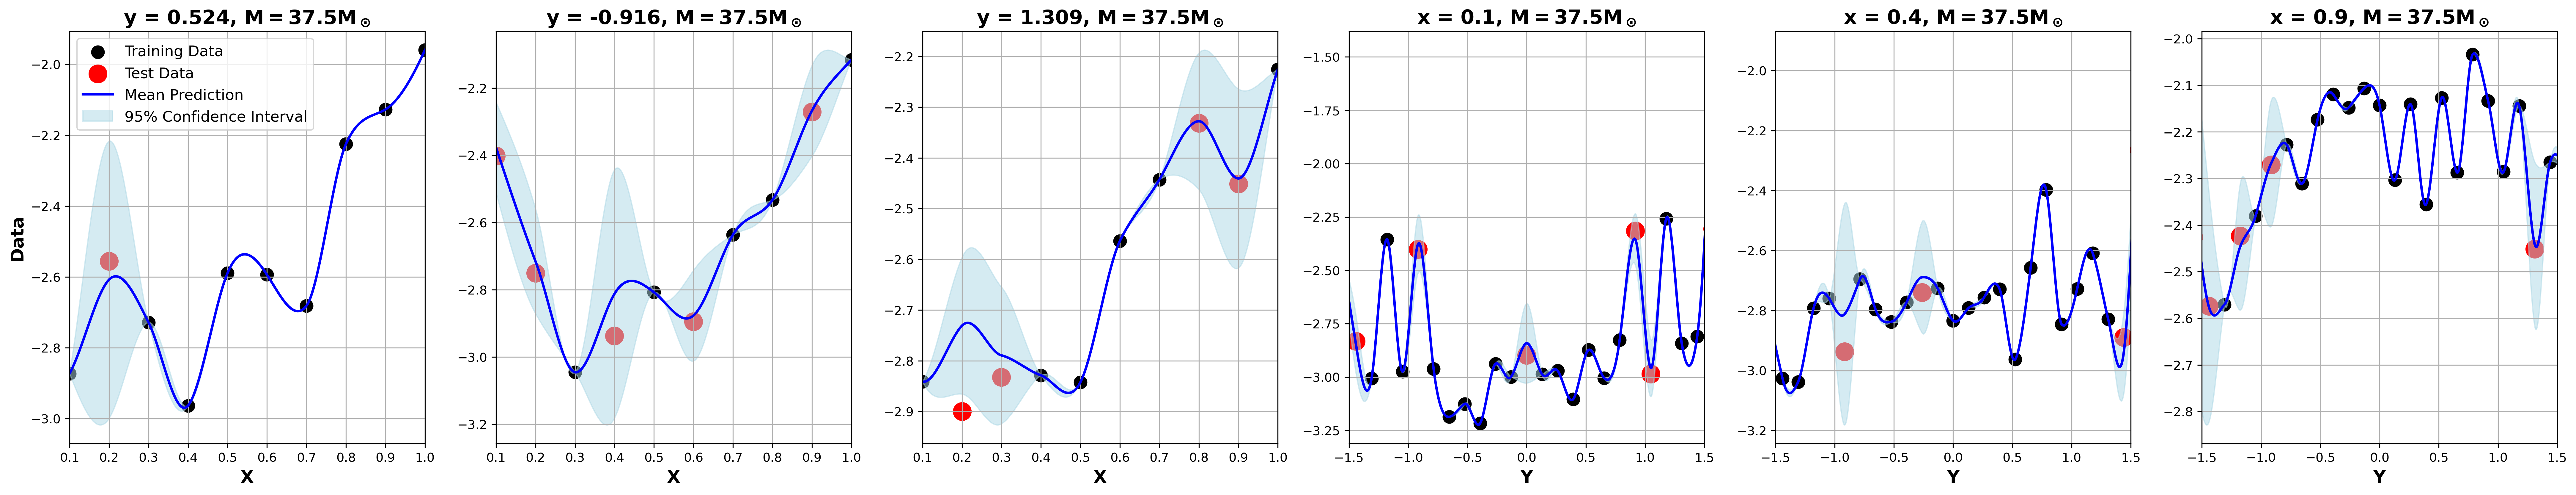
\includegraphics[width=0.8\textwidth]{GoodPlots/No Error.png}  % Change to your image filename
%     \caption{GPR taking into account no error bars}
%     \label{fig:my_graph}
% \end{figure}

% \begin{figure}[H]  % 'H' forces the figure to appear exactly here
%     \centering
%     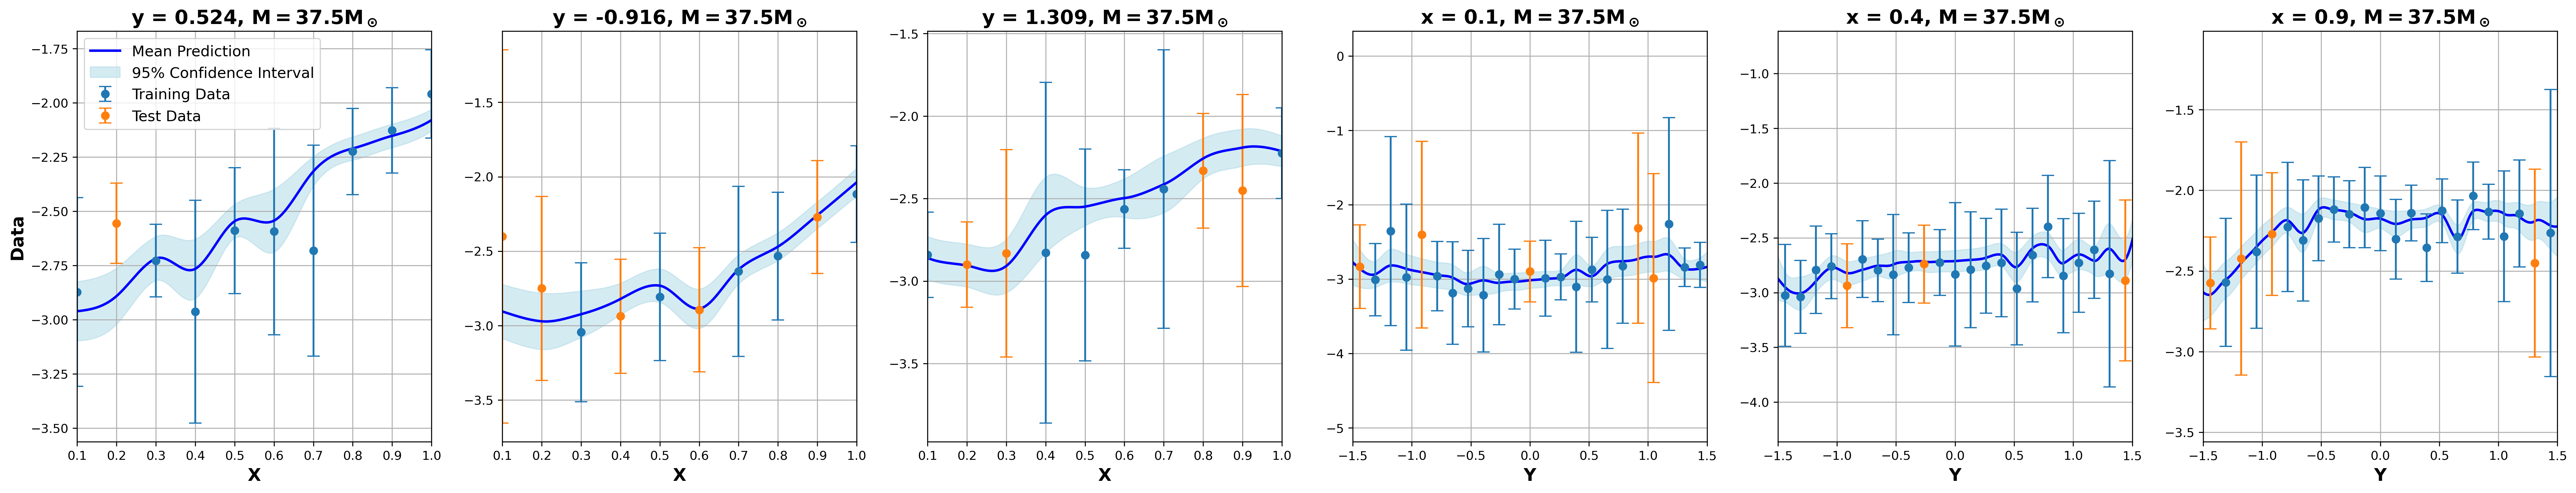
\includegraphics[width=0.8\textwidth]{GoodPlots/Alpha = Err^2.png}  % Change to your image filename
%     \caption{GPR taking error into account on the diagonal of the covariance matrix. Inputing using alpha=$err^2$}
%     \label{fig:my_graph}
% \end{figure}


% \begin{figure}[H]  % 'H' forces the figure to appear exactly here
%     \centering
%     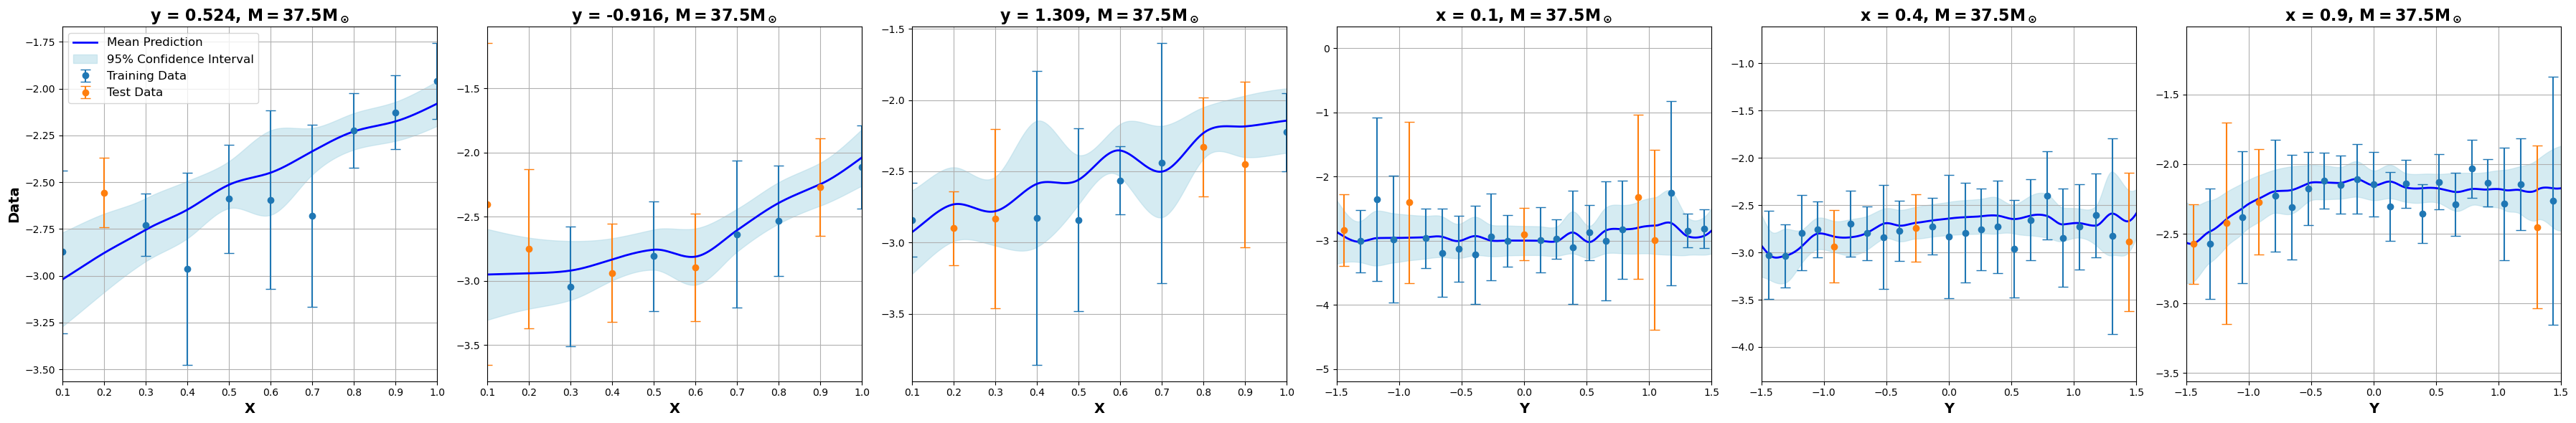
\includegraphics[width=0.8\textwidth]{GoodPlots/Posteriorwithparameterdistribution.png}  % Change to your image filename
%     \caption{Using Alpha=Err^2 and combining this with the posterior distribution of the hyperparameters}
%     \label{fig:my_graph}
% \end{figure}


% \begin{figure}[H]  % 'H' forces the figure to appear exactly here
%     \centering
%     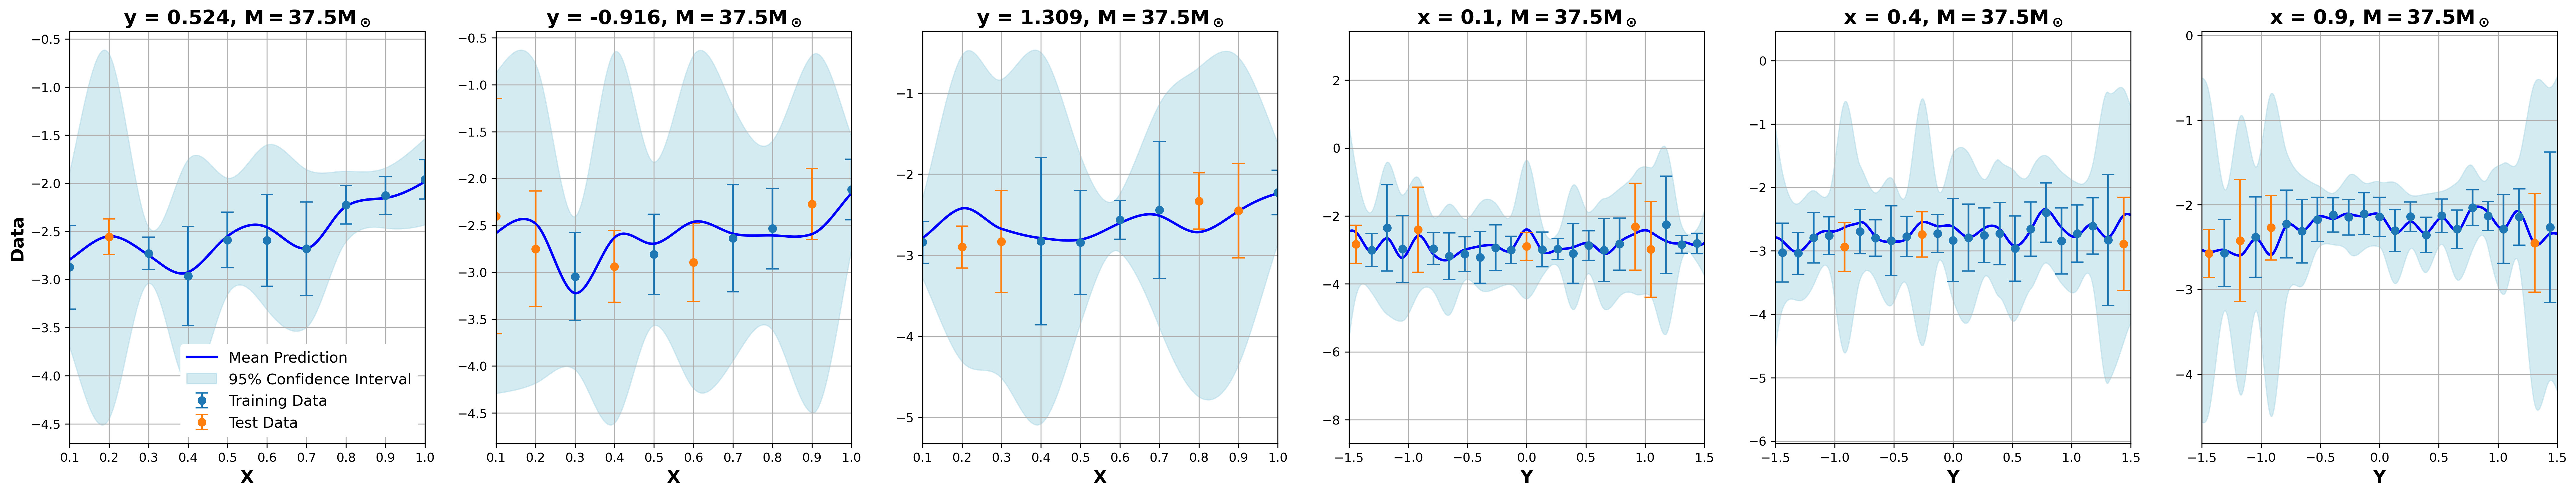
\includegraphics[width=0.8\textwidth]{GoodPlots/Monte Carlo Sampling.png}  % Change to your image filename
%     \caption{Using Monta Carlo sample to sample from true data with error and building mean and credible interval from here}
%     \label{fig:my_graph}
% \end{figure}

% \subsection{Posterior on Hyper-parameter}
% \begin{figure}[H]  % 'H' forces the figure to appear exactly here
%     \centering
%     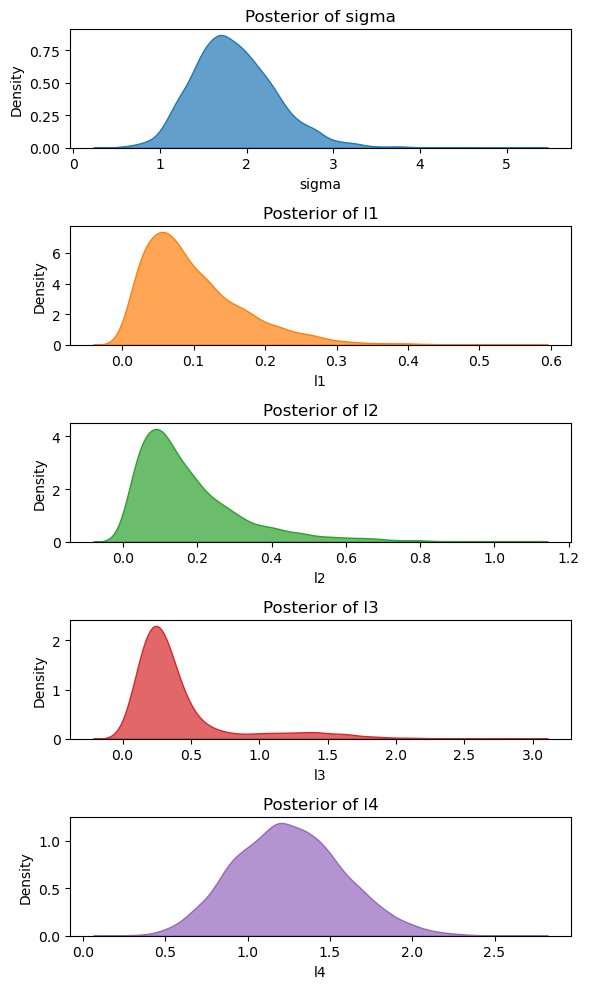
\includegraphics[width=0.8\textwidth]{GoodPlots/Parameter Distribution.png}  % Change to your image filename
%     \caption{Hyper-Parameter Distributions}
%     \label{fig:my_graph}
% \end{figure}


\newpage
\printbibliography
\end{document}

